\documentclass[11pt, british]{beamer}

\usepackage{config}
\usepackage{mathabx}
\usepackage{graphdefs}
\usepackage{pgfplots}
\usepackage{subcaption}
\pgfplotsset{compat=1.13}
\usepgfplotslibrary{statistics}
\newcommand{\norm}[1]{\left\lVert#1\right\rVert}
\usepackage{graphdefs}
\bibliography{lit}

\author{Anton Lorenzen}
\title{Lab Project: Anchored Rectangle Packing}
\date{\today}
\institute{University of Bonn}

\begin{document}

\maketitle

\begin{frame}{The problem}

  \begin{figure}
    \centering
    \begin{subfigure}{4.5cm}
      
\includegraphics[width=4.5cm]{example.png}
    \end{subfigure}%
    \hspace{3mm}%
    \begin{subfigure}{5.5cm}
      \begin{definition}
        Given a finite set of points $P \subset [0,1]^2$,
        find a rectangle $R^p = [p_x, r^p_x) \times [p_y, r^p_y) \subseteq [0,1]^2$ for each $p \in P$
        such that $R^p \cap R^q = \varnothing$ for all $p \neq q \in P$.
        Area: $\sum_{p\in P} (r^p_x - p_x)(r^p_y - p_y)$
      \end{definition}
    \end{subfigure}%
  \end{figure}

  Q: Can you always cover 50\% if $(0,0) \in P$?
\end{frame}

\begin{frame}{Why 50\% ?}
  (interactive)
\end{frame}

\begin{frame}{Contents}
  Algorithmic Approach \\

  Optimal Algorithm through Dynamic Programming \\

  Two Heuristics: \textsc{TilePacking} and \textsc{GreedyPacking} \\

  Different Greedys
\end{frame}

\begin{frame}{Ordering}
  \begin{figure}
    \centering
    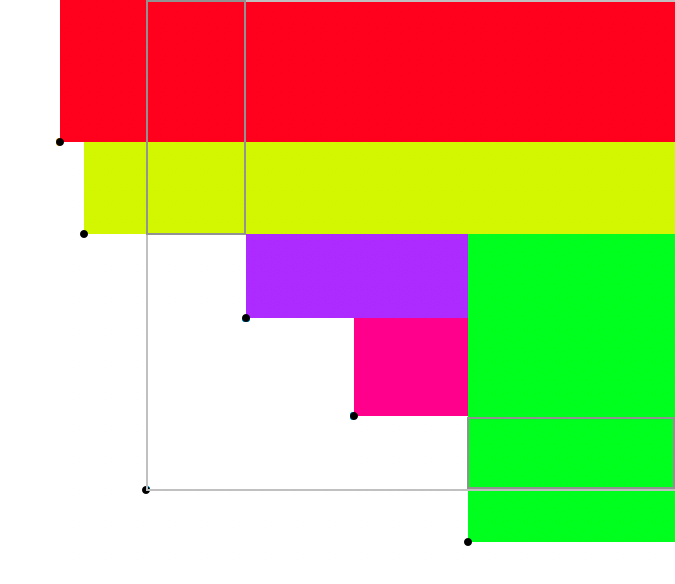
\includegraphics[width=8cm]{precedence 1.png}
  \end{figure}
\end{frame}

\begin{frame}{Ordering}
  \begin{figure}
    \centering
    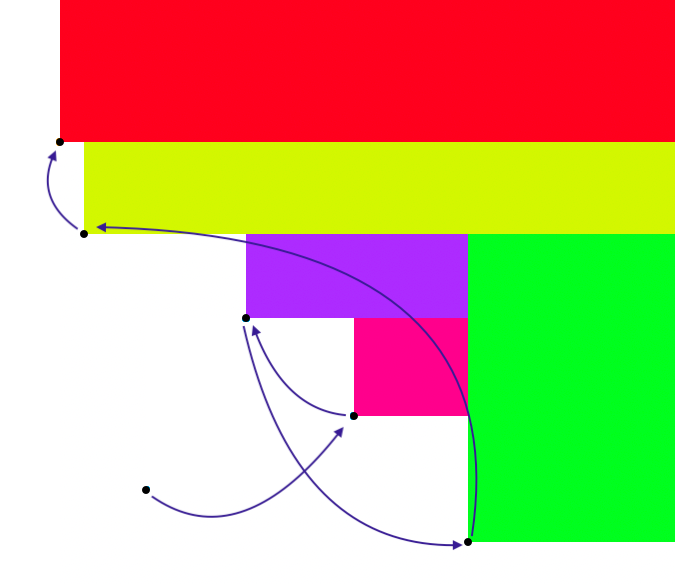
\includegraphics[width=8cm]{precedence 2.png}
  \end{figure}
\end{frame}

\begin{frame}{Tile}
  \begin{figure}
    \centering
    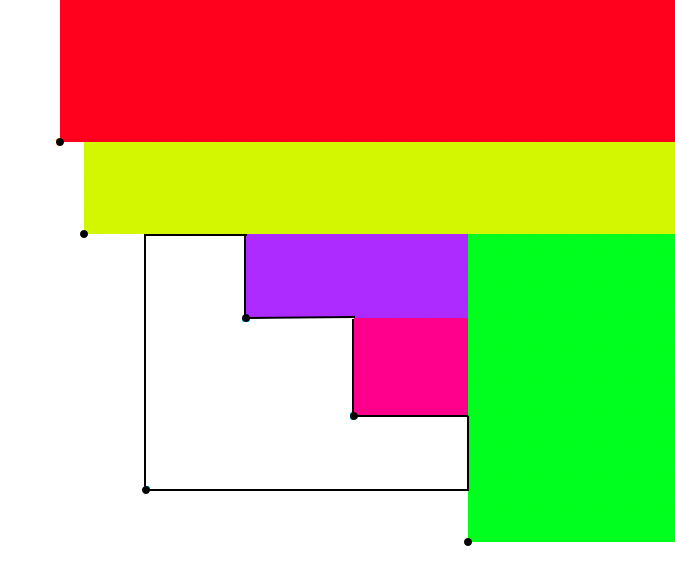
\includegraphics[width=8cm]{tile.png}
  \end{figure}
\end{frame}

\begin{frame}{Greedy Choices}
  \begin{figure}
    \centering
    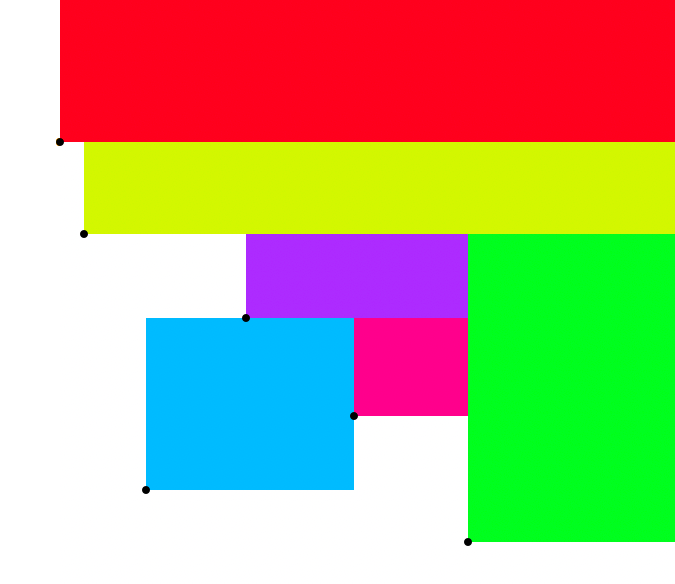
\includegraphics[width=8cm]{greedy-choice.png}
  \end{figure}
\end{frame}

\begin{frame}{Basic Algorithm}
  covered := 0 \\
  For all permutations $\pi$ of $P$, \\
  \phantom{RR} R := pack rectangles greedily in order $\pi$ \\
  \phantom{RR} covered := max(s, coverage(R)) \\
  return covered \\
\end{frame}

\begin{frame}{Dynamic Programming}
  If $\pi = \pi', x$ is the optimal permutation, then $\pi'$ is optimal for $P \setminus \{x\}$. \\

  Idea: Inductively compute $\pi$ for all subsets of $P$. \\

  Held-Karp Dynamic Programming Solver for TSP $O(2^n n\log n)$.
\end{frame}

\begin{frame}{Improving it with Heuristics}
\begin{figure}
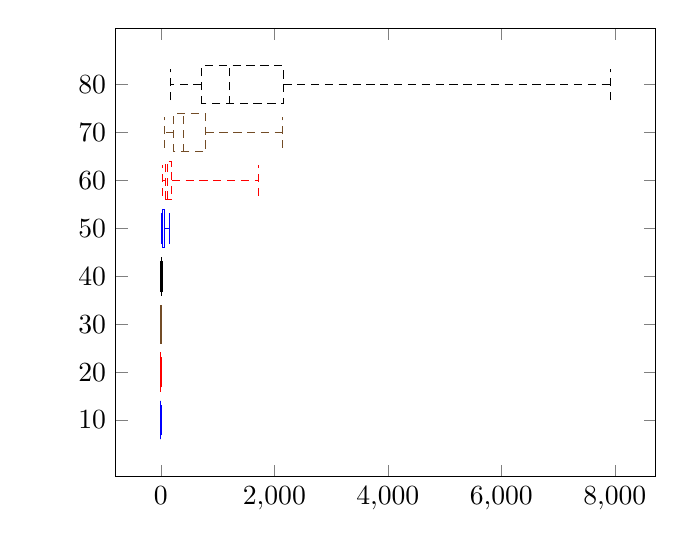
\begin{tikzpicture}
  \begin{axis}% [ boxplot/draw direction=y]
    [
    ytick={1,2,3,4,5,6,7,8},
    yticklabels={10,20,30,40,50,60,70,\phantom{100}80},
    % xtick={1,2,3},
    % xticklabels={Index 0, Index 1, Index 2},
    ]
    \addplot+[
    boxplot prepared={
      median=0,
      upper quartile=0,
      lower quartile=0,
      upper whisker=4,
      lower whisker=0
    },
    ] coordinates {};
    \addplot+[
    boxplot prepared={
      median=0,
      upper quartile=1,
      lower quartile=0,
      upper whisker=4,
      lower whisker=0
    },
    ] coordinates {};
    \addplot+[
    boxplot prepared={
      median=1,
      upper quartile=2,
      lower quartile=1,
      upper whisker=7,
      lower whisker=0
    },
    ] coordinates {};
    \addplot+[
    boxplot prepared={
      median=9,
      upper quartile=14,
      lower quartile=5.75,
      upper whisker=33,
      lower whisker=1
    },
    ] coordinates {};
    \addplot+[
    boxplot prepared={
      median=35.5,
      upper quartile=57,
      lower quartile=24.75,
      upper whisker=157,
      lower whisker=9
    },
    ] coordinates {};
    \addplot+[
    boxplot prepared={
      median=112.5,
      upper quartile=191,
      lower quartile=80.5,
      upper whisker=1720,
      lower whisker=27
    },
    ] coordinates {};
    \addplot+[
    boxplot prepared={
      median=402.5,
      upper quartile=788,
      lower quartile=231,
      upper whisker=2149,
      lower whisker=69
    },
    ] coordinates {};
    \addplot+[
    boxplot prepared={
      median=1208.5,
      upper quartile=2158.75,
      lower quartile=720.75,
      upper whisker=7925,
      lower whisker=171
    },
    ] coordinates {};
  \end{axis}
\end{tikzpicture}
\caption{Time (ms) for the Optimal Algorithm on $n$ uniformly distributed points; 100 instances}
\label{dynprogtime}
\end{figure}
\end{frame}

\begin{frame}{TilePacking}
  Choose a permutation through a sweep and pack accordingly \\

  Easy to implement in time $O(n\log n)$ \\

  Can not cover more than 43\% in some instances
\end{frame}

\begin{frame}{TilePacking: Points}
  \begin{figure}
    \centering
    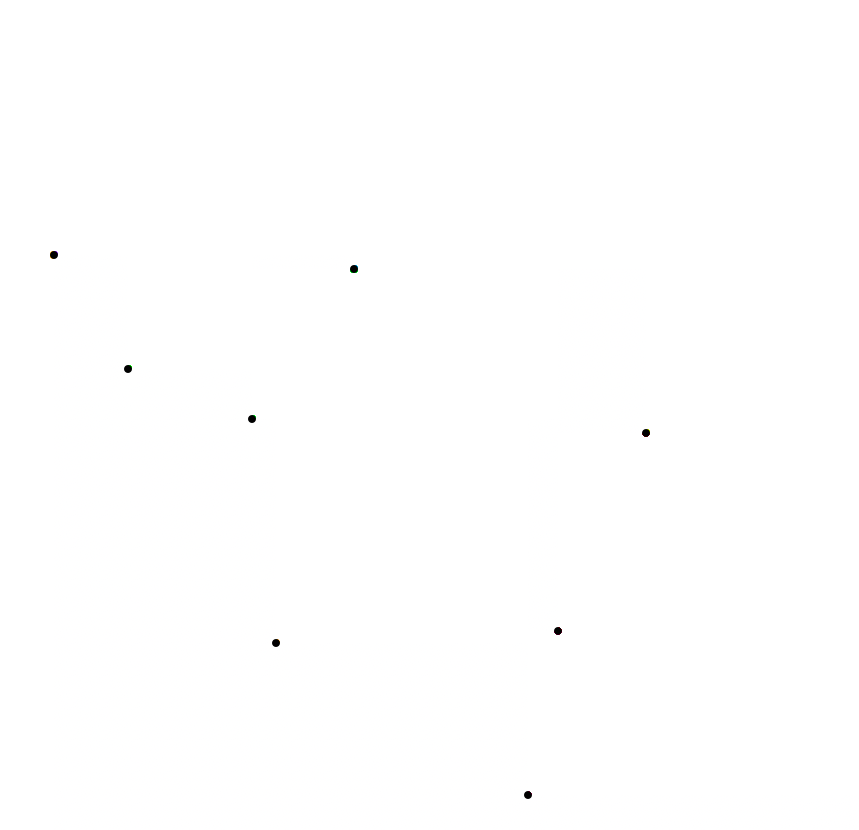
\includegraphics[width=8cm]{points original.png}
  \end{figure}
\end{frame}

\begin{frame}{TilePacking: Permutation}
  \begin{figure}
    \centering
    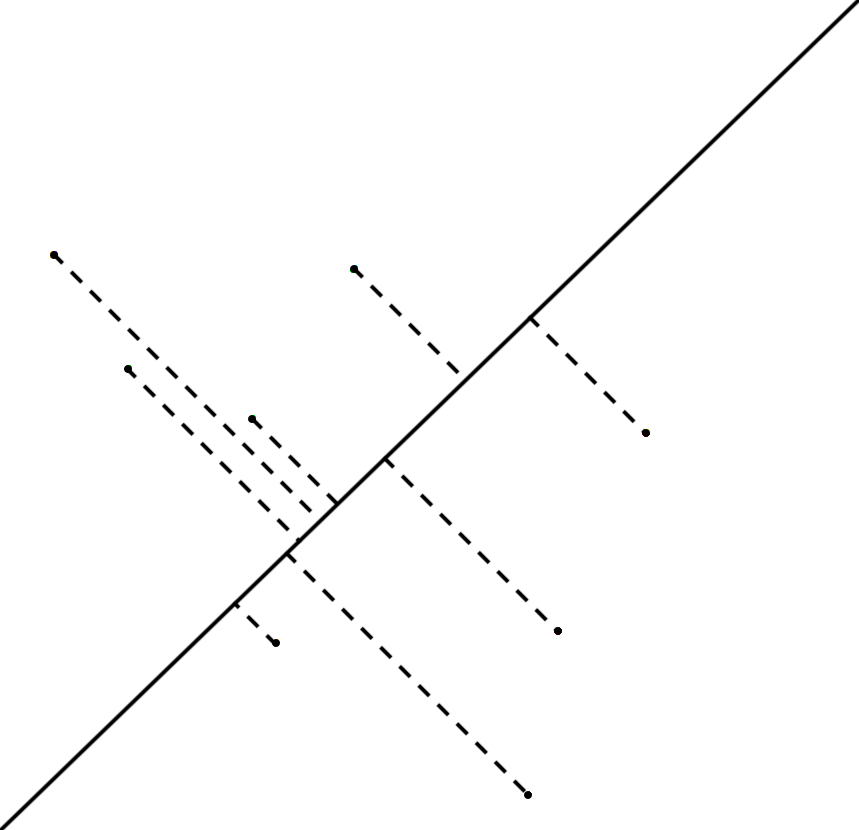
\includegraphics[width=8cm]{points manhattan.png}
  \end{figure}
\end{frame}

\begin{frame}{Problem with TilePacking in Practice}
  (interactive)
\end{frame}

\begin{frame}{Performance in Theory}
  GreedyPacking is no better in theory \\

  Reduction by adding 2 points $(x - \epsilon, y), (x, y - \epsilon)$ for each $(x,y) \in P$ \\

  Corollary: GreedyPacking can not reach 50\% either!
\end{frame}

\begin{frame}{Performance in Practice}
\begin{figure}
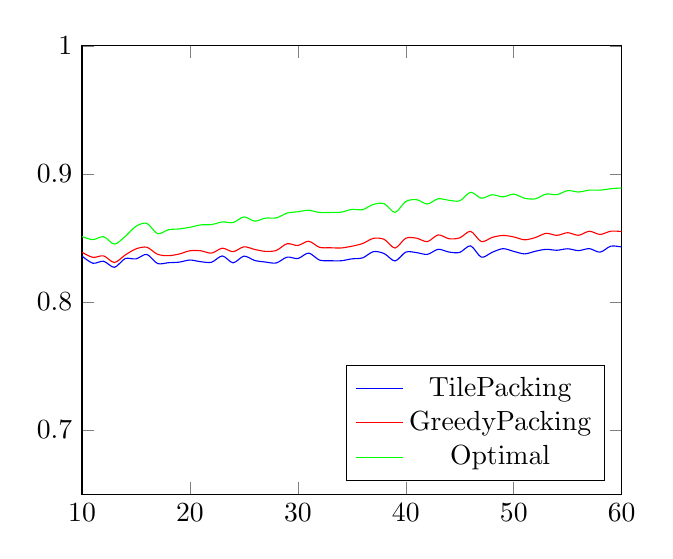
\begin{tikzpicture}
\begin{axis}[
    xmin=10, xmax=60,
    ymin=0.65, ymax=1,
    xtick={10,20,...,60},
    ytick={0.6,0.7,...,1},
    legend pos={south east}
            ]
\addplot[smooth,blue] plot coordinates {
(10, 0.8358224200000001)
(11, 0.8302466879891638)
(12, 0.831807069444444)
(13, 0.827060520710059)
(14, 0.8339054387755103)
(15, 0.8336372400000003)
(16, 0.837162828125)
(17, 0.8300228615916955)
(18, 0.8306620903899115)
(19, 0.8311008676443713)
(20, 0.8327601600000001)
(21, 0.8314543356009068)
(22, 0.8310342251149342)
(23, 0.8359457013232514)
(24, 0.8305785584204619)
(25, 0.8358190447047165)
(26, 0.8324179082840237)
(27, 0.8311753045267491)
(28, 0.8304607155612246)
(29, 0.8350329060642093)
(30, 0.8339311300000002)
(31, 0.8381881560874088)
(32, 0.8327184199218749)
(33, 0.8322249127640035)
(34, 0.8321887474048443)
(35, 0.8336752930612241)
(36, 0.8344445300925929)
(37, 0.8393138619430244)
(38, 0.8377723318524757)
(39, 0.8320292199793965)
(40, 0.8389705200000002)
(41, 0.8385399506246282)
(42, 0.8371745294784576)
(43, 0.8411380827474312)
(44, 0.8389779700413217)
(45, 0.8387166232098764)
(46, 0.8438309692816636)
(47, 0.8349796265278406)
(48, 0.8387871158854169)
(49, 0.8416398021657641)
(50, 0.839513394177135)
(51, 0.8375524401129069)
(52, 0.839606403364963)
(53, 0.841116859380562)
(54, 0.8403799588477371)
(55, 0.8415488829752067)
(56, 0.8400977254464282)
(57, 0.8416742591566634)
(58, 0.8389084916765754)
(59, 0.8436167170353346)
(60, 0.8428993694444447)
};
\addlegendentry{TilePacking}

\addplot[smooth,color=red,]
    plot coordinates {
(10, 0.8388416300000001)
(11, 0.8348412776608068)
(12, 0.8360140069444444)
(13, 0.830833869822485)
(14, 0.8366917602040815)
(15, 0.8414666755555554)
(16, 0.8427527812499997)
(17, 0.8372268269896195)
(18, 0.8361521517265629)
(19, 0.8374489580586325)
(20, 0.8400050424999997)
(21, 0.8399726961451247)
(22, 0.838146205611257)
(23, 0.842018839319471)
(24, 0.839285406365477)
(25, 0.8430901035884539)
(26, 0.8410087973372781)
(27, 0.8395057887517146)
(28, 0.8402413813775506)
(29, 0.8454859024970274)
(30, 0.8441017588888892)
(31, 0.8474300249739855)
(32, 0.8427040439453127)
(33, 0.8423469393939395)
(34, 0.8421738771626298)
(35, 0.8435372253061222)
(36, 0.8456540879629633)
(37, 0.8496994894083271)
(38, 0.848876511261016)
(39, 0.8421262355365513)
(40, 0.8498084918749998)
(41, 0.8497978756692443)
(42, 0.8471361417233558)
(43, 0.8523930048674958)
(44, 0.8493828135330577)
(45, 0.8500671165432103)
(46, 0.8551735170132324)
(47, 0.8471213368039837)
(48, 0.8504128116319443)
(49, 0.8519588567263641)
(50, 0.8507887294602351)
(51, 0.8485557377919929)
(52, 0.8503068154798143)
(53, 0.853621606621573)
(54, 0.8520239626200272)
(55, 0.8540915798347111)
(56, 0.8520598010204087)
(57, 0.8552292880886426)
(58, 0.8527309943519615)
(59, 0.8552863702958917)
(60, 0.8549989750000004)
    };
\addlegendentry{GreedyPacking}

\addplot[smooth,color=green]
    plot coordinates {
(10, 0.8510338399999999)
(11, 0.8486840464612964)
(12, 0.8509638402777775)
(13, 0.8451634378698223)
(14, 0.8511954897959181)
(15, 0.8591045422222221)
(16, 0.86141269140625)
(17, 0.8533048788927338)
(18, 0.8564154781808558)
(19, 0.8570454974639513)
(20, 0.8583204075000004)
(21, 0.86021110430839)
(22, 0.8604233103599739)
(23, 0.8625070207939504)
(24, 0.8620011342783684)
(25, 0.8664330622204863)
(26, 0.8631363520710066)
(27, 0.8654824979423869)
(28, 0.8656389834183674)
(29, 0.8694182175980972)
(30, 0.8704486477777779)
(31, 0.8716256378772111)
(32, 0.8698829931640624)
(33, 0.8699082800734621)
(34, 0.8701298918685122)
(35, 0.8722714555102036)
(36, 0.8720847229938269)
(37, 0.8762043396639885)
(38, 0.8767347858474834)
(39, 0.8699467813904052)
(40, 0.878492593125)
(41, 0.8798533950029744)
(42, 0.8764975379818593)
(43, 0.8806002677122765)
(44, 0.8794083269628098)
(45, 0.8789958844444442)
(46, 0.8856707868620037)
(47, 0.8810120285196921)
(48, 0.8837240108506944)
(49, 0.8820821341107872)
(50, 0.8842262663374848)
(51, 0.8809996949592037)
(52, 0.8805433380241168)
(53, 0.8842874553221788)
(54, 0.8837759489026067)
(55, 0.8869648515702481)
(56, 0.885867488520408)
(57, 0.8873203708833489)
(58, 0.8873194414387636)
(59, 0.8884068190175237)
(60, 0.8890666291666668)
    };
\addlegendentry{Optimal}
\end{axis}
\end{tikzpicture}
\caption{Average coverage of the algorithms on $n$ uniformly random points; 100 instances}
\label{algocov}
\end{figure}
\end{frame}

\begin{frame}{GreedyPacking}
  Best previous algorithm: $O(n^2 \log n)$ time, $O(n^2)$ space \\

  Implemented: $O(n^2)$ time, $O(n)$ space \\

  Described: $O(n \log^2 n + k)$ time, $O(n\log^2 n)$ space
\end{frame}

\begin{frame}{Find Tile Rectangle}
  \begin{figure}
    \centering
    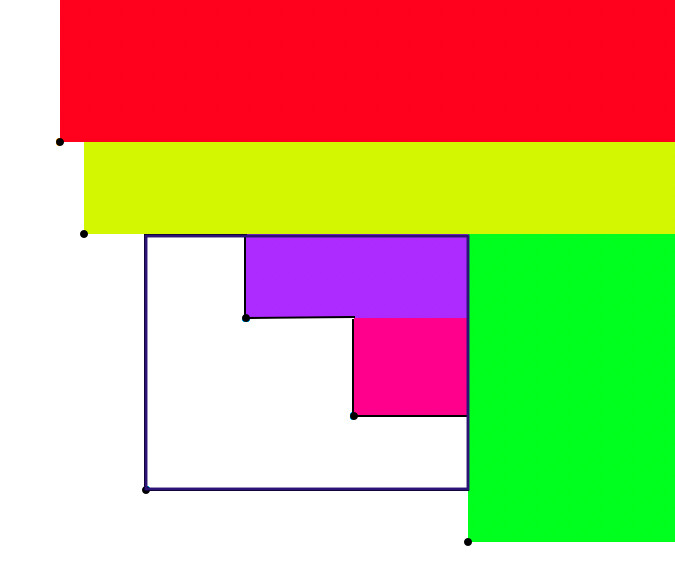
\includegraphics[width=8cm]{tile rectangle.png}
  \end{figure}

  $O(n)$ time, no extra storage
\end{frame}

\begin{frame}{Make greedy choice}
  \begin{figure}
    \centering
    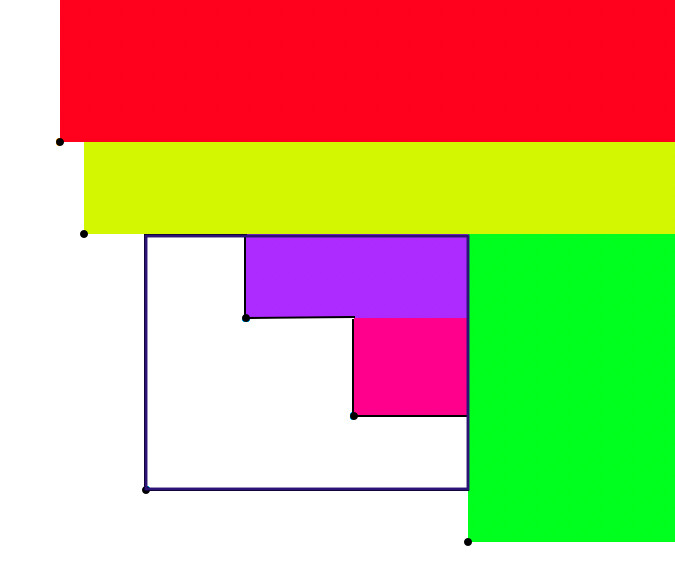
\includegraphics[width=8cm]{tile rectangle.png}
  \end{figure}

  $O(n)$ time, no extra storage \\
  $O(\log^2 n + k)$ time for $k$ points in the tile rect. using a range tree
\end{frame}

\begin{frame}{Find Tile Rectangle (better)}
  \begin{figure}
    \centering
    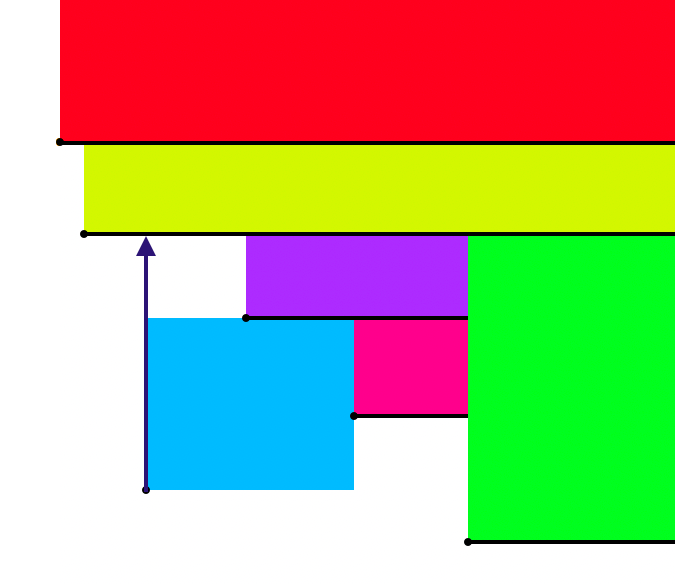
\includegraphics[width=8cm]{ray 1.png}
  \end{figure}

  $O(\log^2 n)$ time using interval and priority search tree 
\end{frame}

\begin{frame}{Find Tile Rectangle (better)}
  \begin{figure}
    \centering
    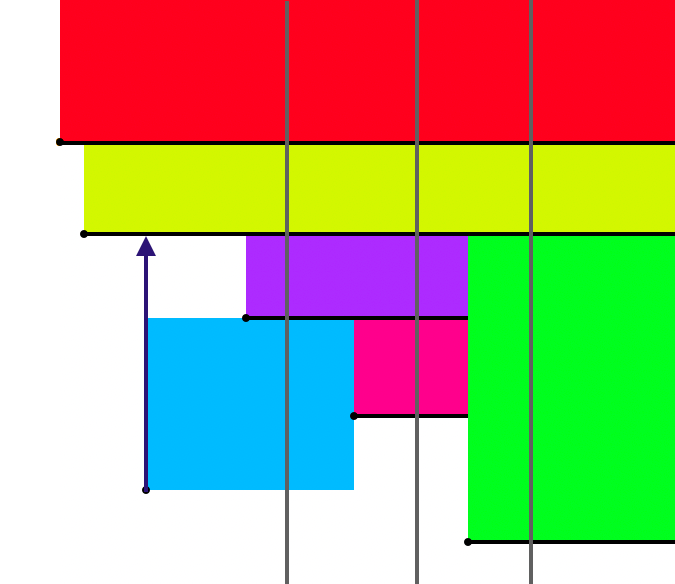
\includegraphics[width=8cm]{ray 3.png}
  \end{figure}

  $O(\log^2 n)$ time using interval and priority search tree 
\end{frame}

\begin{frame}{Find Tile Rectangle (better)}
  \begin{figure}
    \centering
    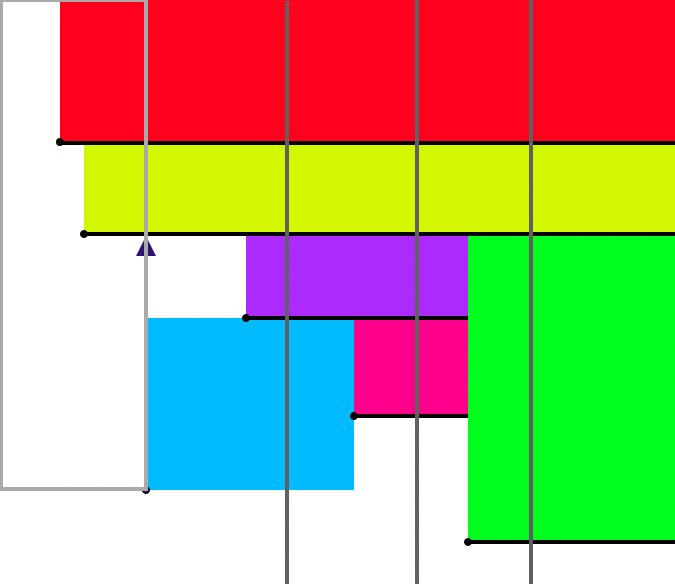
\includegraphics[width=8cm]{ray 4.png}
  \end{figure}

  $O(\log^2 n)$ time using interval and priority search tree 
\end{frame}

\begin{frame}{Solves the TilePacking Problem}
  \begin{figure}
    \centering
    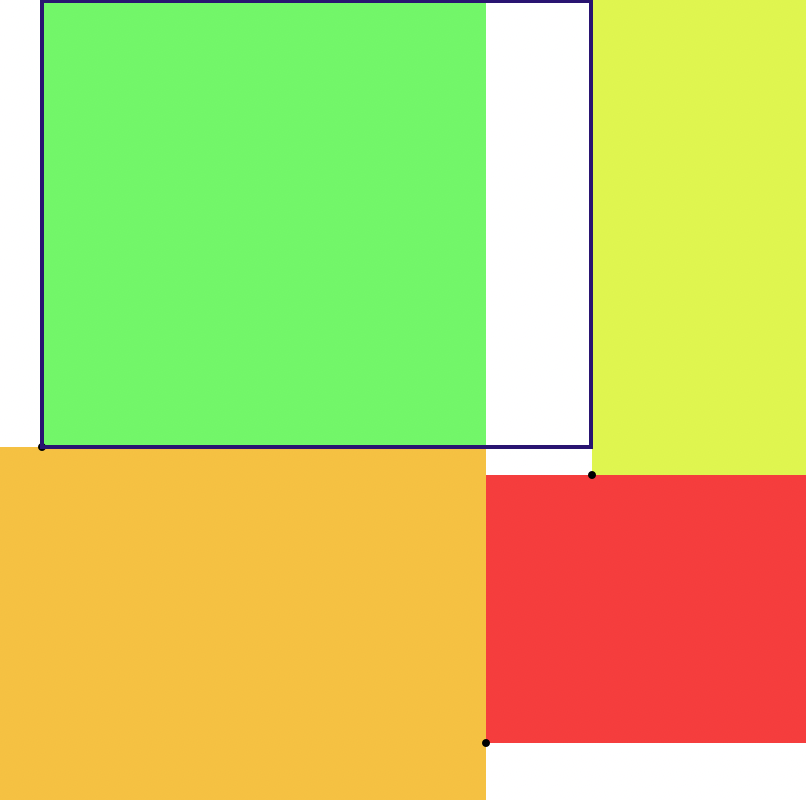
\includegraphics[width=8cm]{problem-tile-packing-revisited.png}
  \end{figure}
\end{frame}

\begin{frame}{GreedyPacking: runtime}
\begin{figure}
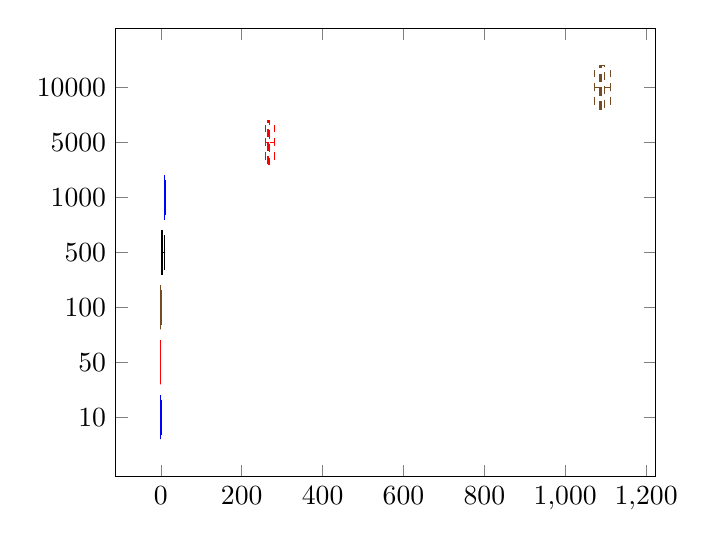
\begin{tikzpicture}
  \begin{axis}% [ boxplot/draw direction=y]
    [
    ytick={1,2,3,4,5,6,7},
    yticklabels={10,50,100,500,1000,5000,10000},
    % xtick={1,2,3},
    % xticklabels={Index 0, Index 1, Index 2},
    ]
    \addplot+[
    boxplot prepared={
      median=0,
      upper quartile=0,
      lower quartile=0,
      upper whisker=2,
      lower whisker=0
    },
    ] coordinates {};
    \addplot+[
    boxplot prepared={
      median=0,
      upper quartile=0,
      lower quartile=0,
      upper whisker=0,
      lower whisker=0
    },
    ] coordinates {};
    \addplot+[
    boxplot prepared={
      median=0,
      upper quartile=0,
      lower quartile=0,
      upper whisker=1,
      lower whisker=0
    },
    ] coordinates {};
    \addplot+[
    boxplot prepared={
      median=2,
      upper quartile=3,
      lower quartile=2,
      upper whisker=10,
      lower whisker=2
    },
    ] coordinates {};
    \addplot+[
    boxplot prepared={
      median=10,
      upper quartile=10,
      lower quartile=9,
      upper whisker=11,
      lower whisker=9
    },
    ] coordinates {};
    \addplot+[
    boxplot prepared={
      median=267,
      upper quartile=269,
      lower quartile=265,
      upper whisker=282,
      lower whisker=259
    },
    ] coordinates {};
    \addplot+[
    boxplot prepared={
      median=1088.5,
      upper quartile=1096,
      lower quartile=1083.75,
      upper whisker=1112,
      lower whisker=1073
    },
    ] coordinates {};
  \end{axis}
\end{tikzpicture}
\caption{Time (ms) for the Greedy Algorithm on $n$ uniformly distributed points; 100 instances}    
\label{greedytime}
\end{figure}
\end{frame}

\begin{frame}{GreedyPacking: Manhattan}
  \begin{figure}
    \centering
    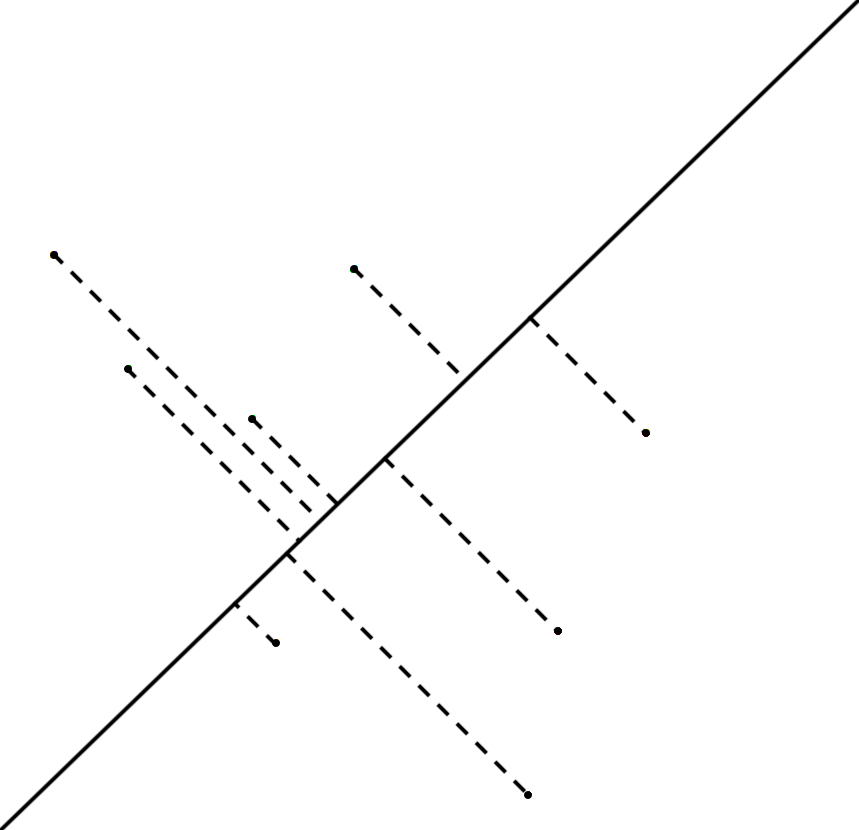
\includegraphics[width=8cm]{points manhattan.png}
  \end{figure}
\end{frame}

\begin{frame}{GreedyPacking: Euclidean}
  \begin{figure}
    \centering
    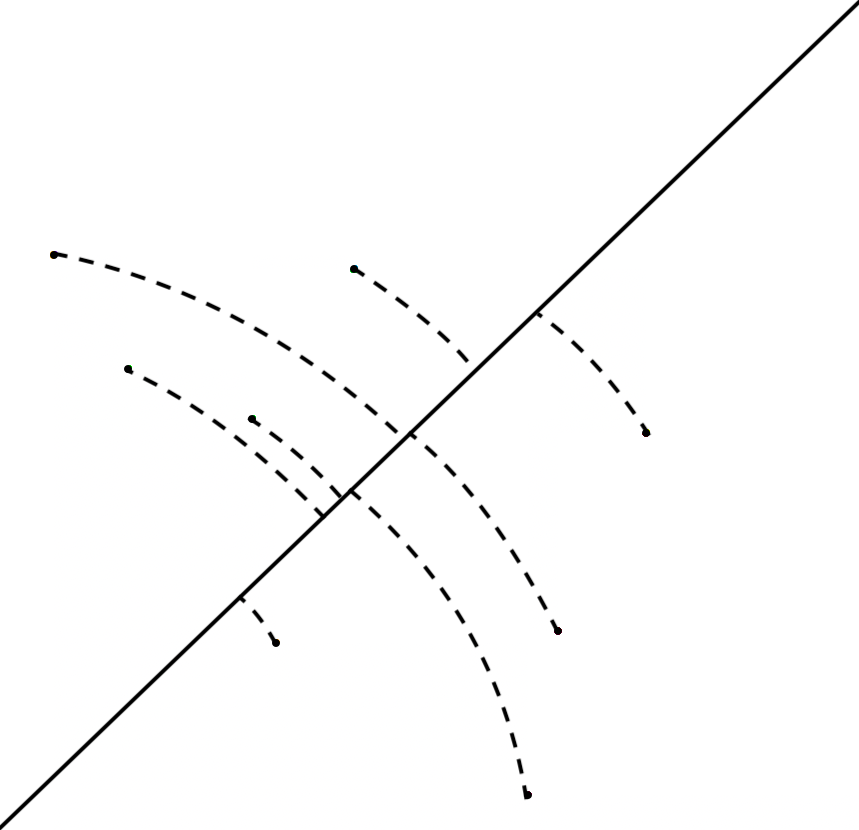
\includegraphics[width=8cm]{points euclidean.png}
  \end{figure}
\end{frame}

\begin{frame}{GreedyPacking: Infinity}
  \begin{figure}
    \centering
    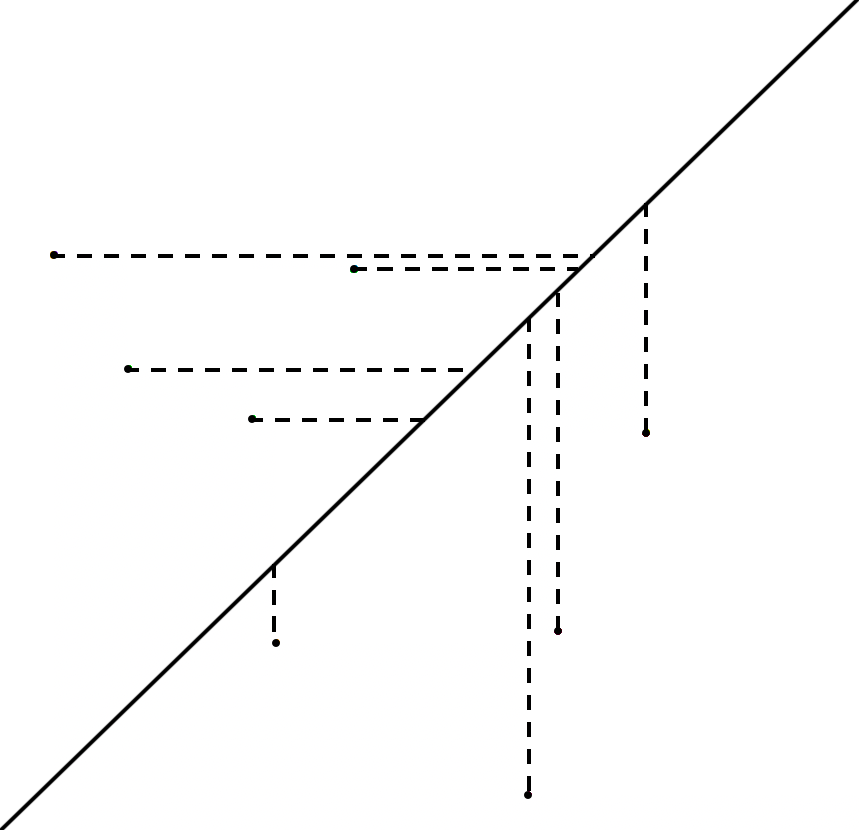
\includegraphics[width=8cm]{points infinity.png}
  \end{figure}
\end{frame}

\begin{frame}{GreedyPacking: Minus Infinity}
  \begin{figure}
    \centering
    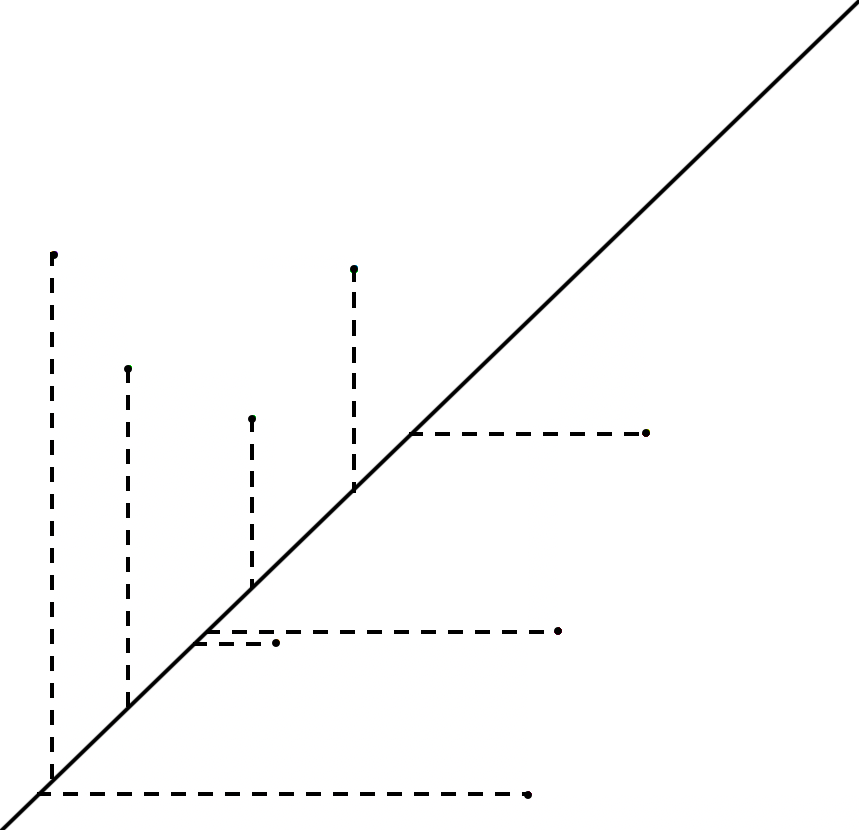
\includegraphics[width=8cm]{points minfinity.png}
  \end{figure}
\end{frame}

\begin{frame}{Norms in Practice}
\begin{figure}
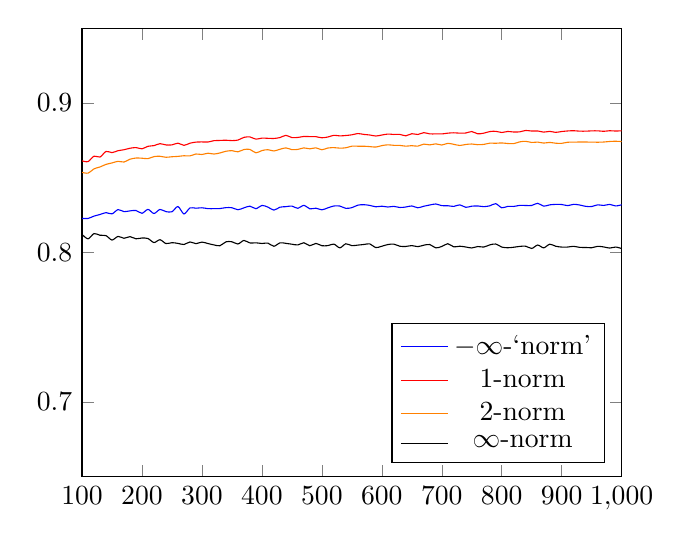
\begin{tikzpicture}
\begin{axis}[
    xmin=100, xmax=1000,
    ymin=0.65, ymax=0.95,
    xtick={100,200,...,1000},
    ytick={0.6,0.7,...,1},
    legend pos={south east}
            ]
\addplot[smooth,blue]
    plot coordinates {
(100, 0.8227174331000005)
(110, 0.8227018329752065)
(120, 0.8242784188194443)
(130, 0.8253559060946749)
(140, 0.8266034440816327)
(150, 0.8257679868888892)
(160, 0.8286226674218748)
(170, 0.8272604011418687)
(180, 0.8277708580246917)
(190, 0.8280345282660377)
(200, 0.8261778813000005)
(210, 0.82877404015873)
(220, 0.8260173873140494)
(230, 0.8287319707561437)
(240, 0.827263008680556)
(250, 0.8271925949480873)
(260, 0.8306726120710058)
(270, 0.8257345037860081)
(280, 0.8297417870918367)
(290, 0.829558807016942)
(300, 0.8298450992)
(310, 0.8292737780020812)
(320, 0.8292475212890623)
(330, 0.8293316547199266)
(340, 0.8299458586591696)
(350, 0.8298760007673468)
(360, 0.8285494952932099)
(370, 0.8297912028341858)
(380, 0.8309241618074791)
(390, 0.8292334750164368)
(400, 0.8314335846687502)
(410, 0.8302955318500896)
(420, 0.8282911452210887)
(430, 0.8302232489021091)
(440, 0.8305916961983474)
(450, 0.8309846282222222)
(460, 0.829482674130435)
(470, 0.831466899791761)
(480, 0.8291266419314235)
(490, 0.8295692325531028)
(500, 0.8284743294977904)
(510, 0.8298068168704349)
(520, 0.83104395662352)
(530, 0.8309988846742605)
(540, 0.8294645428669408)
(550, 0.829932974138843)
(560, 0.8315969237818873)
(570, 0.8319141618005539)
(580, 0.8314157163946748)
(590, 0.8305176739672505)
(600, 0.8308986015416666)
(610, 0.8303734919242142)
(620, 0.8307843380931322)
(630, 0.8300435361577227)
(640, 0.8303586281933594)
(650, 0.8310666462224852)
(660, 0.8298545672038568)
(670, 0.8308787470483405)
(680, 0.8317039352854669)
(690, 0.8323834067989918)
(700, 0.8312612076326529)
(710, 0.8312271459234277)
(720, 0.8307707347627311)
(730, 0.8318157468530686)
(740, 0.8301620117293648)
(750, 0.8309146495751111)
(760, 0.831062092352839)
(770, 0.8305996588227356)
(780, 0.8311390744444445)
(790, 0.8325938270805959)
(800, 0.8298552466828126)
(810, 0.8307743101367887)
(820, 0.8307366915333136)
(830, 0.8314599161147648)
(840, 0.8313722402437645)
(850, 0.8314038116955014)
(860, 0.8328494952244457)
(870, 0.8309223639014925)
(880, 0.8318133540973658)
(890, 0.8321101914265877)
(900, 0.832045941297531)
(910, 0.8312893184446323)
(920, 0.832168554080813)
(930, 0.8316982113816626)
(940, 0.8307973674796281)
(950, 0.8306864038156284)
(960, 0.8318134343869354)
(970, 0.8314053626304605)
(980, 0.8321157579758431)
(990, 0.8310689121991167)
(1000, 0.8318572333510004)
    };
\addlegendentry{$-\infty$-`norm'}

\addplot[smooth,color=red]
    plot coordinates {
(100, 0.8612824981000001)
(110, 0.8607377235537187)
(120, 0.8644076141666669)
(130, 0.8637919683431954)
(140, 0.867554644897959)
(150, 0.8667466357777778)
(160, 0.86804627546875)
(170, 0.8686833904152248)
(180, 0.8696758081790125)
(190, 0.8701368251501909)
(200, 0.8693120798999999)
(210, 0.8709915988662132)
(220, 0.8714380451239673)
(230, 0.8727410950661624)
(240, 0.8718981128298615)
(250, 0.8719248527691421)
(260, 0.8730742431508871)
(270, 0.8716268594650206)
(280, 0.873050564145408)
(290, 0.8737916500974005)
(300, 0.8739067078666669)
(310, 0.8738493574713843)
(320, 0.8747475089453124)
(330, 0.8749064755555556)
(340, 0.8750452694896196)
(350, 0.8748066093469389)
(360, 0.875139828742284)
(370, 0.8769671944119796)
(380, 0.8772497672506924)
(390, 0.8757694171203153)
(400, 0.8764733298250001)
(410, 0.876320729512195)
(420, 0.876237304886621)
(430, 0.8768207949594377)
(440, 0.8783080949535124)
(450, 0.8767986595407408)
(460, 0.876923381904537)
(470, 0.8775811951969219)
(480, 0.8774716154340283)
(490, 0.877432676788838)
(500, 0.8766859042534954)
(510, 0.8772088136332173)
(520, 0.8783287281139053)
(530, 0.8779489991028835)
(540, 0.8782107418141294)
(550, 0.8786705128231405)
(560, 0.8795149565178572)
(570, 0.8789436078578025)
(580, 0.8785500137613101)
(590, 0.8778615420568805)
(600, 0.8785272719722225)
(610, 0.8791752978527277)
(620, 0.8789095247086368)
(630, 0.8789530128168305)
(640, 0.8780020092456051)
(650, 0.8794060373751477)
(660, 0.8788945720890728)
(670, 0.880111742169748)
(680, 0.8792692466500865)
(690, 0.8793065208569628)
(700, 0.8792584342857143)
(710, 0.8797793231521526)
(720, 0.8800220635320217)
(730, 0.8797742285119164)
(740, 0.879871004583638)
(750, 0.8808486113653337)
(760, 0.8793414648337948)
(770, 0.8797729570180466)
(780, 0.880843834975345)
(790, 0.8810153980580033)
(800, 0.8802331919468748)
(810, 0.8809099310056263)
(820, 0.8805413814738252)
(830, 0.8806610365584858)
(840, 0.8815825473228455)
(850, 0.8811863493716264)
(860, 0.8812491422917798)
(870, 0.8804741275938339)
(880, 0.8809618104932849)
(890, 0.8803220795821233)
(900, 0.880872174628395)
(910, 0.8812540962830577)
(920, 0.8814081325177223)
(930, 0.881122474527691)
(940, 0.8811032764169302)
(950, 0.8813158093675859)
(960, 0.8813430602756075)
(970, 0.8810133722829206)
(980, 0.8814000122594754)
(990, 0.8812000767129874)
(1000, 0.881358545207)
    };
\addlegendentry{$1$-norm}

\addplot[smooth,color=orange]
    plot coordinates {
(100, 0.8535563213)
(110, 0.85303339768595)
(120, 0.855903131319445)
(130, 0.8571576531360949)
(140, 0.8588876518877551)
(150, 0.8598419509777784)
(160, 0.8609305835546877)
(170, 0.8604667673010382)
(180, 0.8623509060802468)
(190, 0.8631322804529776)
(200, 0.8630098402750004)
(210, 0.8627541640816329)
(220, 0.864100213512397)
(230, 0.8642989066540647)
(240, 0.8636499606944444)
(250, 0.8639896489415316)
(260, 0.8642360665828399)
(270, 0.8646599315089162)
(280, 0.8645529495025512)
(290, 0.8658233667532086)
(300, 0.865499522511111)
(310, 0.8663505530593131)
(320, 0.8658133439257816)
(330, 0.866532681414141)
(340, 0.8676574989359862)
(350, 0.868064657608163)
(360, 0.867300802631173)
(370, 0.8688256999999999)
(380, 0.8689046103947367)
(390, 0.8666113327481919)
(400, 0.8681230747437502)
(410, 0.8687157127364666)
(420, 0.8678629309297052)
(430, 0.8689852430124391)
(440, 0.869910722035124)
(450, 0.8687504246222223)
(460, 0.8689096136342158)
(470, 0.8699177412449071)
(480, 0.8692886242534719)
(490, 0.8699529885172842)
(500, 0.8686671312697837)
(510, 0.8698230318569777)
(520, 0.8700980934652371)
(530, 0.869749128045568)
(540, 0.8700041811488345)
(550, 0.8710543252793385)
(560, 0.8710449383067598)
(570, 0.8710356061372732)
(580, 0.8707778761869385)
(590, 0.8704841918328067)
(600, 0.8714357510333329)
(610, 0.8719757088255851)
(620, 0.8716389642585848)
(630, 0.8715913224162263)
(640, 0.8710651893823238)
(650, 0.8714194097349113)
(660, 0.8710847459274562)
(670, 0.8724316201715306)
(680, 0.8719381890635814)
(690, 0.8726189081117413)
(700, 0.8718551649959183)
(710, 0.8729563294425712)
(720, 0.8723026507716051)
(730, 0.8715531281459933)
(740, 0.8722060325328715)
(750, 0.8725122805422224)
(760, 0.8720556890200833)
(770, 0.872261326147748)
(780, 0.8730704386900063)
(790, 0.8730176129418363)
(800, 0.8732360936109376)
(810, 0.8728558313948828)
(820, 0.8727742839113621)
(830, 0.8739630963521609)
(840, 0.8743079724121313)
(850, 0.873558291331488)
(860, 0.8737957605137912)
(870, 0.8731464841874887)
(880, 0.8735809192019629)
(890, 0.8730469378702184)
(900, 0.8729791691493831)
(910, 0.8736995683975366)
(920, 0.8737827009676278)
(930, 0.8738469762192157)
(940, 0.8738418830454957)
(950, 0.8737889000595256)
(960, 0.8737160325444875)
(970, 0.8738402118386652)
(980, 0.8742089263567264)
(990, 0.8743651283125236)
(1000, 0.8741586785070004)
    };
\addlegendentry{$2$-norm}

\addplot[smooth,color=black]
    plot coordinates {
(100, 0.8120651392999999)
(110, 0.80906917107438)
(120, 0.8125809496527774)
(130, 0.8114361744378701)
(140, 0.8112210201020409)
(150, 0.8082605975555552)
(160, 0.8106942185937502)
(170, 0.8094390829757786)
(180, 0.810520357067901)
(190, 0.8090974939215283)
(200, 0.8096185293999997)
(210, 0.8092510970748299)
(220, 0.8065766443388429)
(230, 0.8084681815689982)
(240, 0.8059013950347221)
(250, 0.806494640440844)
(260, 0.8060182658727802)
(270, 0.8052802024142665)
(280, 0.806969782015306)
(290, 0.8058399659479012)
(300, 0.8068879649333333)
(310, 0.8059119339958377)
(320, 0.8049933800878907)
(330, 0.8044424527180902)
(340, 0.8070632728546714)
(350, 0.8070999999265308)
(360, 0.8056205555092594)
(370, 0.8079845999488682)
(380, 0.8063132401731303)
(390, 0.8064060966206444)
(400, 0.8059548931625002)
(410, 0.8061827857168353)
(420, 0.8041098016439908)
(430, 0.8063919585343424)
(440, 0.8060291654028923)
(450, 0.8054658376592593)
(460, 0.8049828448393196)
(470, 0.8064266785694884)
(480, 0.8044677546397568)
(490, 0.8059812679966681)
(500, 0.8044693599366097)
(510, 0.8045267461168781)
(520, 0.8055473645118343)
(530, 0.8030511735920257)
(540, 0.8057444588511657)
(550, 0.8045133977454545)
(560, 0.8048650204591836)
(570, 0.8052857795567867)
(580, 0.8056734309459916)
(590, 0.8031901525624826)
(600, 0.8041187151861116)
(610, 0.8052454413356622)
(620, 0.8055327318444324)
(630, 0.8041163735802475)
(640, 0.8039658064306643)
(650, 0.8045435222295856)
(660, 0.8038393574977043)
(670, 0.8048133692091781)
(680, 0.8052512192863318)
(690, 0.8030113090359167)
(700, 0.8039548953693877)
(710, 0.805787495006943)
(720, 0.8037085869347996)
(730, 0.8041203831244134)
(740, 0.803610472878013)
(750, 0.8029596452639999)
(760, 0.8039192717468832)
(770, 0.8035556160448639)
(780, 0.8050100802005252)
(790, 0.8055973875308446)
(800, 0.8035608026843755)
(810, 0.8030982606729359)
(820, 0.8034468702111834)
(830, 0.8039969320767496)
(840, 0.8041274655187073)
(850, 0.8026350196359863)
(860, 0.8049029871444026)
(870, 0.8030301684669419)
(880, 0.805472313926911)
(890, 0.8041004685178639)
(900, 0.8035542099777778)
(910, 0.8035730652421207)
(920, 0.8040615064331287)
(930, 0.8033399709134001)
(940, 0.8032963278372566)
(950, 0.8031007133986086)
(960, 0.804058656905382)
(970, 0.8036490368105008)
(980, 0.8028896070803835)
(990, 0.8035643885629397)
(1000, 0.8025622500970002)
    };
\addlegendentry{$\infty$-norm}
\end{axis}
\end{tikzpicture}
\caption{Average coverage of the greedy algorithm on $n$ uniformly random points; 100 instances}
\label{normcov}
\end{figure}
\end{frame}

\begin{frame}{Why are other norms interesting?}

  No norm is better than any other! \\

  Damerius found no counter-example for the $(-)\infty$-norms \\

\end{frame}

\begin{frame}{Interactive}

\end{frame}

\begin{frame}{Questions?}

\end{frame}

% \begin{frame}{Reference Counting for Functional Languages}
    % \begin{itemize}[label=-]
        % \item Memory reclamation: Unused data magically goes away
        % \item Two approaches: Garbage Collector vs. Reference Counting
        % \item Generational Garbage Collection "won": Haskell, OCaml, many more
    % \end{itemize}
% \end{frame}

% \begin{frame}{Contents}
    % \begin{itemize}[label=-]
        % \item Reference Counting
        % \item Precise Placement of Reference Count Instructions
        % \item Reuse 
        % \item Benchmarks
        % \item Linear Resource Calculus (and $\star$-condition)
        % \item Other optimizations
        % \item Functional But In-Place
    % \end{itemize}
% \end{frame}

% \begin{frame}{Why Reference Counting for Functional Languages?}
    % \begin{itemize}[label=-]
        % \item Reference counting is a memory management technique
        % \item Implemented in Swift, Python,... but not Haskell, OCaml
        % % \item Haskell, OCaml etc use generational garbage collection
    % \end{itemize}
    % \vspace{2cm}
    % This talk: Use reference counting to achieve
    % \begin{itemize}[label=-]
      % \item provably minimal space usage
      % \item good performance
    % \end{itemize}
% \end{frame}

% \begin{frame}{What is Reference Counting?}
% \begin{figure}
  % \centering
   % \scalebox{0.8}{
    % \begin{tikzpicture}
    % \tikzstyle{stackvar}=[node distance = 0mm, minimum size = 10mm]
    % \draw[step=1cm,gray,thin] (6.7,0) grid (12,1);
    % \node[stackvar] (z) at (11.5, 0.5) {x};
    % \draw[thick] (6.3,-0.3) -- (13.2,-0.3) node[anchor=north] {heap} node[anchor=south] {stack};
    % \tikzstyle{node}=[draw, node distance = 15mm, minimum size = 7mm]
    % \node[node] (d1) at (11.5, -1.3) {}; 
    % \node[node] (d2) [below right of=d1] {}; 
    % \node[node] (d3) [below left of=d1] {}; 
    % \node[node] (d4) [below left of=d2] {}; 
    % \draw[->] (z) -- (d1);
    % \draw[->] (d1) -- (d2);
    % \draw[->] (d1) -- (d3);
    % \draw[->] (d2) -- (d4);
    % \draw[->] (d3) -- (d4);
    % \end{tikzpicture}
  % }
% \end{figure}
% \end{frame}

% \begin{frame}{What is Reference Counting?}
% \begin{figure}
  % \centering
   % \scalebox{0.8}{
    % \begin{tikzpicture}
    % \tikzstyle{stackvar}=[node distance = 0mm, minimum size = 10mm]
    % \draw[step=1cm,gray,thin] (6.7,0) grid (12,1);
    % \node[stackvar] (z) at (11.5, 0.5) {x};
    % \draw[thick] (6.3,-0.3) -- (13.2,-0.3) node[anchor=north] {heap} node[anchor=south] {stack};
    % \tikzstyle{node}=[draw, node distance = 15mm, minimum size = 7mm]
    % \node[node] (d1) at (11.5, -1.3) {1}; 
    % \node[node] (d2) [below right of=d1] {1}; 
    % \node[node] (d3) [below left of=d1] {1}; 
    % \node[node] (d4) [below left of=d2] {2}; 
    % \draw[->] (z) -- (d1);
    % \draw[->] (d1) -- (d2);
    % \draw[->] (d1) -- (d3);
    % \draw[->] (d2) -- (d4);
    % \draw[->] (d3) -- (d4);
    % \end{tikzpicture}
  % }
% \end{figure}
% \end{frame}

% \begin{frame}{What is Reference Counting?}
% \begin{figure}
  % \centering
   % \scalebox{0.8}{
    % \begin{tikzpicture}
    % \tikzstyle{stackvar}=[node distance = 0mm, minimum size = 10mm]
    % \draw[step=1cm,gray,thin] (6.7,0) grid (12,1);
    % \node[stackvar] (z) at (11.5, 0.5) {x};
    % \draw[thick] (6.3,-0.3) -- (13.2,-0.3) node[anchor=north] {heap} node[anchor=south] {stack};
    % \tikzstyle{node}=[draw, node distance = 15mm, minimum size = 7mm]
    % \node[node] (d1) at (11.5, -1.3) {0}; 
    % \node[node] (d2) [below right of=d1] {1}; 
    % \node[node] (d3) [below left of=d1] {1}; 
    % \node[node] (d4) [below left of=d2] {2}; 
    % \draw[->] (d1) -- (d2);
    % \draw[->] (d1) -- (d3);
    % \draw[->] (d2) -- (d4);
    % \draw[->] (d3) -- (d4);
    % \end{tikzpicture}
  % }
% \end{figure}
% \end{frame}

% \begin{frame}{What is Reference Counting?}
% \begin{figure}
  % \centering
   % \scalebox{0.8}{
    % \begin{tikzpicture}
    % \tikzstyle{stackvar}=[node distance = 0mm, minimum size = 10mm]
    % \draw[step=1cm,gray,thin] (6.7,0) grid (12,1);
    % \node[stackvar] (z) at (11.5, 0.5) {x};
    % \draw[thick] (6.3,-0.3) -- (13.2,-0.3) node[anchor=north] {heap} node[anchor=south] {stack};
    % \tikzstyle{node}=[draw, node distance = 15mm, minimum size = 7mm]
    % \tikzstyle{ghost}=[draw, node distance = 15mm, minimum size = 7mm, color = white]
    % \node[ghost] (d1) at (11.5, -1.3) {x}; 
    % \node[node] (d2) [below right of=d1] {0}; 
    % \node[node] (d3) [below left of=d1] {0}; 
    % \node[node] (d4) [below left of=d2] {2}; 
    % \draw[->] (d2) -- (d4);
    % \draw[->] (d3) -- (d4);
    % \end{tikzpicture}
  % }
% \end{figure}
% \end{frame}

% \begin{frame}{What is Reference Counting?}
% \begin{figure}
  % \centering
   % \scalebox{0.8}{
    % \begin{tikzpicture}
    % \tikzstyle{stackvar}=[node distance = 0mm, minimum size = 10mm]
    % \draw[step=1cm,gray,thin] (6.7,0) grid (12,1);
    % \node[stackvar] (z) at (11.5, 0.5) {x};
    % \draw[thick] (6.3,-0.3) -- (13.2,-0.3) node[anchor=north] {heap} node[anchor=south] {stack};
    % \tikzstyle{node}=[draw, node distance = 15mm, minimum size = 7mm]
    % \tikzstyle{ghost}=[draw, node distance = 15mm, minimum size = 7mm, color = white]
    % \node[ghost] (d1) at (11.5, -1.3) {x}; 
    % \node[ghost] (d2) [below right of=d1] {x}; 
    % \node[ghost] (d3) [below left of=d1] {x}; 
    % \node[node] (d4) [below left of=d2] {0}; 
    % \end{tikzpicture}
  % }
% \end{figure}
% \end{frame}

% \begin{frame}{What is Reference Counting?}
% \begin{figure}
  % \centering
   % \scalebox{0.8}{
    % \begin{tikzpicture}
    % \tikzstyle{stackvar}=[node distance = 0mm, minimum size = 10mm]
    % \draw[step=1cm,gray,thin] (6.7,0) grid (12,1);
    % \node[stackvar] (z) at (11.5, 0.5) {x};
    % \draw[thick] (6.3,-0.3) -- (13.2,-0.3) node[anchor=north] {heap} node[anchor=south] {stack};
    % \tikzstyle{node}=[draw, node distance = 15mm, minimum size = 7mm]
    % \tikzstyle{ghost}=[draw, node distance = 15mm, minimum size = 7mm, color = white]
    % \node[ghost] (d1) at (11.5, -1.3) {x}; 
    % \node[ghost] (d2) [below right of=d1] {x}; 
    % \node[ghost] (d3) [below left of=d1] {x}; 
    % \node[ghost] (d4) [below left of=d2] {0}; 
    % \end{tikzpicture}
  % }
% \end{figure}
% \end{frame}

% \begin{frame}[fragile]{Reference Count Instructions}
% \begin{code}
% fun dup(x)
  % x.refcount += 1

% fun drop(x)
  % if x.refcount == 1
    % then map(drop, x.children); free(x)
    % else x.refcount -= 1
% \end{code}
% \end{frame}

% \begin{frame}[fragile]{Updating Reference Counts: Example}
% \begin{code}
% fun map(f : a -> b, xs : list<a>) : list<b>
  % match xs 
    % Cons(x, xx) -> Cons(f(x), map(f, xx))
    % Nil -> Nil

% fun main()
  % let xs = list(1, 10000)
  % let ys = map(fn(x) {x + 1}, xs)
  % print(ys)
% \end{code}
% \end{frame}


% \begin{frame}[fragile]{1. Idea: Drop when falling out of lexical scope}
% \begin{code}
% fun map(f : a -> b, xs : list<a>) : list<b>
  % match xs 
    % Cons(x, xx) -> Cons(f(x), map(f, xx))
    % Nil -> Nil

% fun main()
  % let xs = list(1, 10000)
  % let ys = map(fn(x) {x + 1}, xs)
  % print(ys)
  % drop(xs)
  % drop(ys)
% \end{code}
% \end{frame}

% % \begin{frame}[fragile]{Updating Reference Counts}
  % % Key idea: Pass values into functions \\

  % % \vspace{1cm}

% % \end{frame}

% \begin{frame}[fragile]{2. Idea: Pass ownership of values into functions}
% \begin{code}
% fun map(f : a -> b, xs : list<a>) : list<b>
  % match xs 
    % Cons(x, xx) ->
      % dup(x); dup(xx); drop(xs)
      % Cons(f(x), map(f, xx))
    % Nil -> Nil

% fun main()
  % let xs = list(1, 10000)
  % let ys = map(fn(x) {x + 1}, xs)
  % print(ys)
% \end{code}
% \end{frame}

% \begin{frame}[fragile]{\textit{Precise} Reference Counting is better!}
  % \begin{itemize}[label=-]
    % \item More dup/drop overall
    % \item Dup/dropped variable likely in cache
    % \item Uses only half as much space in the example!
  % \end{itemize}
  % \vspace{1cm}
  % See: $[$Beans$], [$Perceus$]$
  % % $[$Counting Immutable Beans; Ullrich, de Moura$]$ \\
  % % $[$Perceus: Garbage Free Reference Counting with Reuse; \\
  % % Reinking, Xie, de Moura, Leijen$]$
% \end{frame}

% \begin{frame}[fragile]{Drop specialisation}
% \begin{code}
% fun map(f : a -> b, xs : list<a>) : list<b>
  % match xs 
    % Cons(x, xx) ->
      % dup(x); dup(xx); 
      % if xs.refcount == 1
        % then drop(x); drop(xx); free(xs)
        % else xs.refcount -= 1
      % Cons(f(x), map(f, xx))
    % Nil -> Nil

% fun main()
  % let xs = list(1, 10000)
  % let ys = map(fn(x) {x + 1}, xs)
  % print(ys)
% \end{code}
% \end{frame}

% \begin{frame}[fragile]{Drop specialisation}
% \begin{code}
% fun map(f : a -> b, xs : list<a>) : list<b>
  % match xs 
    % Cons(x, xx) ->
      % if xs.refcount == 1
        % then free(xs)
        % else dup(x); dup(xx); xs.refcount -= 1
      % Cons(f(x), map(f, xx))
    % Nil -> Nil

% fun main()
  % let xs = list(1, 10000)
  % let ys = map(fn(x) {x + 1}, xs)
  % print(ys)
% \end{code}
% \end{frame}

% \begin{frame}[fragile]{Reuse analysis}
% \begin{code}
% fun map(f : a -> b, xs : list<a>) : list<b>
  % match xs 
    % Cons(x, xx) ->
      % let ru = if xs.refcount == 1
        % then &xs; 
        % else dup(x); dup(xx);
             % xs.refcount -= 1; NULL
      % Cons@ru(f(x), map(f, xx))
    % Nil -> Nil

% fun main()
  % let xs = list(1, 10000)
  % let ys = map(fn(x) {x + 1}, xs)
  % print(ys)
% \end{code}
% \end{frame}

% \begin{frame}[fragile]{Reuse analysis is great!}
  % \begin{itemize}[label=-]
    % \item Only half as much allocation as before in the example
    % \item In-place mutation for unique (refcount == 1) values
  % \end{itemize}
  % \vspace{1cm}
  % See: $[$Beans$], [$Perceus$]$
  % % $[$Counting Immutable Beans; Ullrich, de Moura$]$ \\
  % % $[$Perceus: Garbage Free Reference Counting with Reuse; \\
  % % Reinking, Xie, de Moura, Leijen$]$
% \end{frame}

% \begin{frame}[fragile]{Benchmarks}
  % 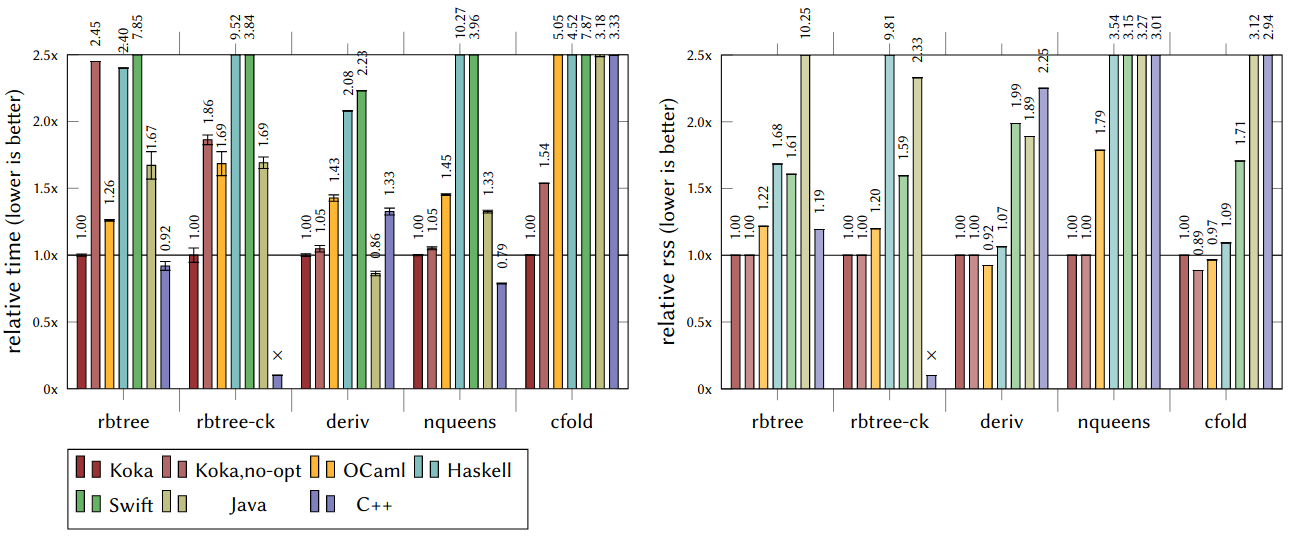
\includegraphics[width=11.5cm]{perceus_benchmark_wide.png} \\
  % See: $[$Perceus$]$
  % % $[$Perceus: Garbage Free Reference Counting with Reuse; \\
  % % Reinking, Xie, de Moura, Leijen$]$
% \end{frame}

% \begin{frame}[fragile]{Other optimizations}
  % \begin{itemize}[label=-]
    % \item Reuse needs precision
    % \item Deferred refcounts and coalescing cannot work with reuse
    % \item Borrowing as a static version of coalescing
  % \end{itemize}
  % \vspace{1cm}
  % See: $[$Beans$], [$Masterthesis$]$
  % % $[$Minimizing Reference Count Updating with Deferred and Anchored \\
  % % Pointers for Functional Data Structures; Baker$]$ \\
  % % $[$Counting Immutable Beans; Ullrich, de Moura$]$ \\
  % % $[$Optimizing Reference Counting with Borrowing; Lorenzen$]$ \\
% \end{frame}

% \begin{frame}[fragile]{Key ideas}
  % \begin{itemize}[label=-]
    % \item Pass ownership of values into functions
    % \item Use \textit{precise} placement of refcount instructions to reduce space usage
    % \item Reuse unused memory spots for new allocations
  % \end{itemize}
  % \vspace{0.7cm}
  % Any Questions? \\
  % Up next: How to do the precise placement \\
% \end{frame}

% \begin{frame}[fragile]{Linear Resource Calculus}
  % \begin{center}
    % \AxiomC{\phantom{N}}
    % \RightLabel{var}
    % \UnaryInfC{$\Delta \mid x \then x \red x$}
    % \DisplayProof
    % \hspace{0.5cm}
    % \AxiomC{$\Delta,x \mid \Gamma \then e \red e'$}
    % \RightLabel{app}
    % \UnaryInfC{$\Delta \mid \Gamma, x \then e\;x \red e'\;x$}
    % \spacedProof
    % % \AxiomC{$\Delta \mid \Gamma, x \then e \red e'$}
    % % \AxiomC{$x \in \Delta, \Gamma$}
    % % \RightLabel{dup}
    % % \BinaryInfC{$\Delta \mid \Gamma \then e \red \dup x;\; e'$}
    % % \DisplayProof
    % % \hspace{0.2cm}
    % % \AxiomC{$\Delta \mid \Gamma \then e \red e'$}
    % % \RightLabel{drop}
    % % \UnaryInfC{$\Delta \mid \Gamma, x \then e \red \drop x;\; e'$}
    % % \spacedProof
    % % \AxiomC{$\Delta \mid \Gamma,r \then e \red e'$}
    % % \RightLabel{drop-reuse}
    % % \UnaryInfC{$\Delta \mid \Gamma, x \then e \red \text{drop-reuse}\;x;\;e'$}
    % % \DisplayProof
    % \AxiomC{\phantom{N}}
    % \RightLabel{con}
    % \UnaryInfC{$\Delta \mid x_1 \dots x_n \then C\,x_1 \dots x_n \red C\,x_1 \dots x_n$}
    % \spacedProof
    % % \AxiomC{$\varnothing \mid \Gamma, x \then e \red e'$}
    % % \AxiomC{$\Gamma = \text{free variables of } \lambda x,\,e$}
    % % \RightLabel{lam}
    % % \BinaryInfC{$\Delta \mid \Gamma \then \lambda x,\,e \red \lambda^\Gamma x,\,e'$}
    % % \spacedProof
    % % \AxiomC{$\Delta \mid \Gamma, \text{bv}(p_i) \then e_i \red e'_i$}
    % % \AxiomC{$x \in \Delta, \Gamma$}
    % % \RightLabel{match}
    % % \BinaryInfC{$\Delta \mid \Gamma \then \match\;x\;\{\overline{p_i \rightarrow e_i}\} \red \match\;x\;\{\overline{p_i \rightarrow \dup \text{bv}(p_i);\; e'_i}\}$}
    % % \spacedProof
    % % \AxiomC{$x \notin \Delta, \Gamma_1, \Gamma_2$}
    % % \AxiomC{$\Delta, \Gamma_2 \mid \Gamma_1 \then e_1 \red e'_1$}
    % % \AxiomC{$\Delta \mid \Gamma_2, x \then e_2 \red e'_2$}
    % % \AxiomC{$(\star)$}
    % % \RightLabel{val}
    % % \QuaternaryInfC{$\Delta \mid \Gamma_1, \Gamma_2 \then \val\;x = e_1;\; e_2 \red \val\;x = e'_1;\; e'_2$}
    % % \DisplayProof
  % \end{center}
  % \vspace{2cm}
  % % $[$Perceus: Garbage Free Reference Counting with Reuse; \\
  % % Reinking, Xie, de Moura, Leijen$]$
  % See: $[$Perceus$]$
% \end{frame}

% \begin{frame}[fragile]{Linear Resource Calculus}
  % \begin{center}
    % % \AxiomC{\phantom{N}}
    % % \RightLabel{var}
    % % \UnaryInfC{$\Delta \mid x \then x \red x$}
    % % \DisplayProof
    % % \hspace{0.5cm}
    % % \AxiomC{$\Delta,x \mid \Gamma \then e \red e'$}
    % % \RightLabel{app}
    % % \UnaryInfC{$\Delta \mid \Gamma, x \then e\;x \red e'\;x$}
    % % \spacedProof
    % \AxiomC{$\Delta \mid \Gamma, x \then e \red e'$}
    % \AxiomC{$x \in \Delta, \Gamma$}
    % \RightLabel{dup}
    % \BinaryInfC{$\Delta \mid \Gamma \then e \red \dup x;\; e'$}
    % \spacedProof
    % \AxiomC{\phantom{{\Huge I}} $\Delta \mid \Gamma \then e \red e'$}
    % \RightLabel{drop}
    % \UnaryInfC{$\Delta \mid \Gamma, x \then e \red \drop x;\; e'$}
    % \spacedProof
    % % \AxiomC{$\Delta \mid \Gamma,r \then e \red e'$}
    % % \RightLabel{drop-reuse}
    % % \UnaryInfC{$\Delta \mid \Gamma, x \then e \red \text{drop-reuse}\;x;\;e'$}
    % % \DisplayProof
    % % \AxiomC{\phantom{N}}
    % % \RightLabel{con}
    % % \UnaryInfC{$\Delta \mid x_1 \dots x_n \then C\,x_1 \dots x_n \red C\,x_1 \dots x_n$}
    % % \spacedProof
    % % \AxiomC{$\varnothing \mid \Gamma, x \then e \red e'$}
    % % \AxiomC{$\Gamma = \text{free variables of } \lambda x,\,e$}
    % % \RightLabel{lam}
    % % \BinaryInfC{$\Delta \mid \Gamma \then \lambda x,\,e \red \lambda^\Gamma x,\,e'$}
    % % \spacedProof
    % % \AxiomC{$\Delta \mid \Gamma, \text{bv}(p_i) \then e_i \red e'_i$}
    % % \AxiomC{$x \in \Delta, \Gamma$}
    % % \RightLabel{match}
    % % \BinaryInfC{$\Delta \mid \Gamma \then \match\;x\;\{\overline{p_i \rightarrow e_i}\} \red \match\;x\;\{\overline{p_i \rightarrow \dup \text{bv}(p_i);\; e'_i}\}$}
    % % \spacedProof
    % % \AxiomC{$x \notin \Delta, \Gamma_1, \Gamma_2$}
    % % \AxiomC{$\Delta, \Gamma_2 \mid \Gamma_1 \then e_1 \red e'_1$}
    % % \AxiomC{$\Delta \mid \Gamma_2, x \then e_2 \red e'_2$}
    % % \AxiomC{$(\star)$}
    % % \RightLabel{val}
    % % \QuaternaryInfC{$\Delta \mid \Gamma_1, \Gamma_2 \then \val\;x = e_1;\; e_2 \red \val\;x = e'_1;\; e'_2$}
    % % \DisplayProof
  % \end{center}
% \end{frame}

% \begin{frame}[fragile]{Linear Resource Calculus}
  % \begin{center}
    % % \AxiomC{\phantom{N}}
    % % \RightLabel{var}
    % % \UnaryInfC{$\Delta \mid x \then x \red x$}
    % % \DisplayProof
    % % \hspace{0.5cm}
    % % \AxiomC{$\Delta,x \mid \Gamma \then e \red e'$}
    % % \RightLabel{app}
    % % \UnaryInfC{$\Delta \mid \Gamma, x \then e\;x \red e'\;x$}
    % % \spacedProof
    % % \AxiomC{$\Delta \mid \Gamma, x \then e \red e'$}
    % % \AxiomC{$x \in \Delta, \Gamma$}
    % % \RightLabel{dup}
    % % \BinaryInfC{$\Delta \mid \Gamma \then e \red \dup x;\; e'$}
    % % \DisplayProof
    % % \hspace{0.2cm}
    % % \AxiomC{$\Delta \mid \Gamma \then e \red e'$}
    % % \RightLabel{drop}
    % % \UnaryInfC{$\Delta \mid \Gamma, x \then e \red \drop x;\; e'$}
    % % \spacedProof
    % % \AxiomC{$\Delta \mid \Gamma,r \then e \red e'$}
    % % \RightLabel{drop-reuse}
    % % \UnaryInfC{$\Delta \mid \Gamma, x \then e \red \text{drop-reuse}\;x;\;e'$}
    % % \DisplayProof
    % % \AxiomC{\phantom{N}}
    % % \RightLabel{con}
    % % \UnaryInfC{$\Delta \mid x_1 \dots x_n \then C\,x_1 \dots x_n \red C\,x_1 \dots x_n$}
    % % \spacedProof
    % % \AxiomC{$\varnothing \mid \Gamma, x \then e \red e'$}
    % % \AxiomC{$\Gamma = \text{free variables of } \lambda x,\,e$}
    % % \RightLabel{lam}
    % % \BinaryInfC{$\Delta \mid \Gamma \then \lambda x,\,e \red \lambda^\Gamma x,\,e'$}
    % % \spacedProof
    % % \AxiomC{$\Delta \mid \Gamma, \text{bv}(p_i) \then e_i \red e'_i$}
    % % \AxiomC{$x \in \Delta, \Gamma$}
    % % \RightLabel{match}
    % % \BinaryInfC{$\Delta \mid \Gamma \then \match\;x\;\{\overline{p_i \rightarrow e_i}\} \red \match\;x\;\{\overline{p_i \rightarrow \dup \text{bv}(p_i);\; e'_i}\}$}
    % % \spacedProof
    % \AxiomC{$\Delta, \Gamma_2 \mid \Gamma_1 \then e_1 \red e'_1$}
    % \noLine
    % \UnaryInfC{$\Delta \mid \Gamma_2, x \then e_2 \red e'_2$}
    % \AxiomC{$x \notin \Delta, \Gamma_1, \Gamma_2$}
    % \noLine
    % \UnaryInfC{$(\star)$}
    % \RightLabel{val}
    % \BinaryInfC{$\Delta \mid \Gamma_1, \Gamma_2 \then \val\;x = e_1;\; e_2 \red \val\;x = e'_1;\; e'_2$}
    % \DisplayProof
  % \end{center}
  % \vspace{2cm}
  % See: $[$Frame Limited$]$
  % % $[$Reference Counting with Frame Limited Reuse; \\
  % % Lorenzen, Leijen$]$
% \end{frame}

% \begin{frame}[fragile]{Garbage Free}
  % \begin{center}
    % \AxiomC{$\Delta, \Gamma_2 \mid \Gamma_1 \then e_1 \red e'_1$}
    % \noLine
    % \UnaryInfC{$\Delta \mid \Gamma_2, x \then e_2 \red e'_2$}
    % \AxiomC{$x \notin \Delta, \Gamma_1, \Gamma_2$}
    % \noLine
    % \UnaryInfC{$\Gamma_2 \subseteq \text{fv}(e_2)$}
    % \RightLabel{val}
    % \BinaryInfC{$\Delta \mid \Gamma_1, \Gamma_2 \then \val\;x = e_1;\; e_2 \red \val\;x = e'_1;\; e'_2$}
    % \DisplayProof
  % \end{center}
  % \vspace{1cm}
  % An evaluation $\varnothing \mid e \red^*_r H \mid x$ is called garbage-free iff for every intermediate
  % state $H_i \mid E[v]$ in the evaluation, we have that for all $y \in \text{dom}(H_i), \text{reach}(y, H_i \mid E[v])$.\\
  % \vspace{1cm}

  % See: $[$Perceus$]$
  % % $[$Perceus: Garbage Free Reference Counting with Reuse; \\
  % % Reinking, Xie, de Moura, Leijen$]$
% \end{frame}

% \begin{frame}[fragile]{Frame Limited}
  % \begin{center}
    % \AxiomC{$\Delta, \Gamma_2 \mid \Gamma_1 \then e_1 \red e'_1$}
    % \noLine
    % \UnaryInfC{$\Delta \mid \Gamma_2, x \then e_2 \red e'_2$}
    % \AxiomC{$x \notin \Delta, \Gamma_1, \Gamma_2$}
    % \noLine
    % \UnaryInfC{$\Gamma_2 = \Gamma' \cup \Gamma'', \Gamma' \subseteq \text{fv}(e_2), \text{sizeof}(\Gamma'') \leq c$}
    % \RightLabel{val}
    % \BinaryInfC{$\Delta \mid \Gamma_1, \Gamma_2 \then \val\;x = e_1;\; e_2 \red \val\;x = e'_1;\; e'_2$}
    % \DisplayProof
  % \end{center}
  % \vspace{1cm}
  % An evaluation $\varnothing \mid e \red^*_r H \mid x$ is called frame-limited iff for every intermediate
  % state $H_i \mid E[v]$ in the evaluation, we have that $H_i = H_1, H_2$ such that for all $y \in \text{dom}(H_1), \text{reach}(y, H_i \mid E[v])$
  % and $|H_2| \leq c \cdot |E|$ for some constant $c$. \\
  % % An evaluation ∅ | e ′ ↦ −→∗r H | x is called frame-limited iff for every intermediate state Hi | E[v ] in
% % the evaluation, we have that Hi equals H1, H2 such that for all y ∈ dom(H1), reach(y, H1 | ⌈E[v ]⌉)
% % and |H2 | ⩽ c · |E| for some constant c.
  % \vspace{1cm}

  % See: $[$Frame Limited$]$
  % % $[$Reference Counting with Frame Limited Reuse; \\
  % % Lorenzen, Leijen$]$
% \end{frame}

% \begin{frame}[fragile]{Reuse analysis}
% \begin{code}
% fun map(f : a -> b, xs : list<a>) : list<b>
  % match xs 
    % Cons(x, xx) ->
      % let ru = if xs.refcount == 1
        % then &xs; 
        % else dup(x); dup(xx);
             % xs.refcount -= 1; NULL
      % Cons@ru(f(x), map(f, xx))
    % Nil -> Nil

% fun main()
  % let xs = list(1, 10000)
  % let ys = map(fn(x) {x + 1}, xs)
  % print(ys)
% \end{code}
% \end{frame}

% \begin{frame}[fragile]{Key ideas}
  % \begin{itemize}[label=-]
    % \item Use a linear calculus to pass ownership
    % \item Weakening: drop / Contraction: dup
    % \item Garbage-free: Every object in memory still reachable
    % \item Use the $\star$-condition to connect formal properties to memory usage
  % \end{itemize}
% \end{frame}

% \begin{frame}{Literature}
    % \begin{itemize}[label=-]
        % \item Counting Immutable Beans (IFL 2019) \\
        % Sebastian Ullrich, Leonardo de Moura
        % \item Perceus: Garbage Free Reference Counting with Reuse \\
        % (PLDI 2021, distinguished paper award) \\
        % Alex Reinking, Ningning Xie, Leo de Moura, Daan Leijen
        % \item Reference Counting with Frame Limited Reuse (Draft) \\
        % Anton Lorenzen, Daan Leijen
        % \item Optimizing Reference Counting with Borrowing \\
        % (my Master Thesis, supervised by Daan Leijen) 
    % \end{itemize}
    % \vspace{0.7cm}
    % Feel free to email me: anfelor@posteo.de
% \end{frame}

% \begin{frame}[fragile]{Bonus: Functional But In-Place}
% \begin{code}
% fun map(f : a -> b, xs : list<a>) : list<b>
  % match xs 
    % Cons(x, xx) -> Cons(f(x), map(f, xx))
    % Nil -> Nil

% fun map-acc(f : a -> b, xs : list<a>,
            % k : list<b>)
  % match xs 
    % Cons(x, xx) -> map-acc(f, xx, Cons(x, k))
    % Nil -> reverse(k)
% \end{code}
% \end{frame}

% \begin{frame}[fragile]{Functional But In-Place}
% \begin{code}
% fun map(f : a -> b, xs : list<a>) : list<b>
  % match xs 
    % Cons(x, xx) -> Cons(f(x), map(f, xx))
    % Nil -> Nil

% fun map-cps(f : a -> b, xs : list<a>,
            % k : list<b> -> list<b>)
  % match xs 
    % Cons(x, xx) ->
      % let fx = f(x)
      % map-cps(f, xx, fn(fxx) {Cons(fx, fxx)})
    % Nil -> k(Nil)
% \end{code}
% \end{frame}

% \begin{frame}[fragile]{Functional But In-Place}
% \begin{code}
% fun map-cps(f : a -> b, xs : list<a>,
            % k : list<b> -> list<b>)
  % match xs 
    % Cons(x, xx) ->
      % let fx = f(x)
      % map-cps(f, xx, fn(fxx) {Cons(fx, fxx)})
    % Nil -> k(Nil)

% fun map-def(f : a -> b, xs : list<a>,
            % k : list<b>)
  % match xs 
    % Cons(x, xx) ->
      % let fx = f(x)
      % map-def(f, xx, Cons(f(x), k))
    % Nil -> reverse(k)
% \end{code}
% \end{frame}

% \begin{frame}[fragile]{Functional But In-Place}
  % \begin{itemize}[label=-]
    % \item Use Continuation-Passing-Style to avoid stackframes
    % \item If the data is unique, you do not have to allocate closures!
    % \item "Imperative" algorithms under-the-hood
    % \item Applies widely: red-black tree insertion better than Okasaki!
  % \end{itemize}
  % \vspace{1cm}
  % See: $[$Recycling continuations, Jonathan Sobel, Daniel Friedman$]$ \\
  % $[$Perceus$], [$Frame Limited$], [$Masterthesis$]$
  % % $[$Perceus: Garbage Free Reference Counting with Reuse \\
  % % Alex Reinking, Ningning Xie, Leo de Moura, Daan Leijen$]$
  % % $[$Optimizing Reference Counting with Borrowing, Anton Lorenzen$]$ \\
% \end{frame}

% % \begin{frame}{Literature}
    % % \begin{itemize}[label=-]
        % % \item Counting Immutable Beans (IFL 2019) \\
        % % Sebastian Ullrich, Leonardo de Moura
        % % \item Perceus: Garbage Free Reference Counting with Reuse \\
        % % (PLDI 2021, distinguished paper award) \\
        % % Alex Reinking, Ningning Xie, Leo de Moura, Daan Leijen
        % % \item Reference Counting with Frame Limited Reuse (Draft) \\
        % % Anton Lorenzen, Daan Leijen
        % % \item Optimizing Reference Counting with Borrowing \\
        % % (my Master Thesis, supervised by Daan Leijen) 
    % % \end{itemize}
    % % \vspace{0.7cm}
    % % Feel free to email me: anfelor@posteo.de
% % \end{frame}

% % \begin{frame}[fragile]{Scope-based Reference Counting}
% % \begin{cpp}
% % int foo(std::shared_ptr<std::vector<int>> v) {
    % % do_something(v);
    % % allocate_a_lot();
    % % // v.~shared_ptr<std::vector<int>>();
% % }
% % \end{cpp}
% % \end{frame}

% % \begin{frame}{Reference Counting: Atomic Reference Counts}
    % % \begin{itemize}[label=-]
      % % \item Atomics are slow, but faster than in the past
      % % (programs will take 1.2x-1.7x more time)
      % % \item Use non-atomic refcounts by default
      % % \item Special function to make objects thread-shared
      % % that converts refcounts to atomics.
    % % \end{itemize}
% % \end{frame}

% % \begin{frame}{Reference Counting: Cycles}
    % % \begin{itemize}[label=-]
      % % \item Uncommon in functional programming
      % % \item Cycle Collectors exist (e.g. Bacon's work)
    % % \end{itemize}
% % \end{frame}

% % \begin{frame}[fragile]{Scope-based Reference Counting}
% % \begin{cpp}
% % int foo(std::shared_ptr<std::vector<int>> v) {
    % % do_something(v);
    % % allocate_a_lot();
    % % // v.~shared_ptr<std::vector<int>>();
% % }
% % \end{cpp}
% % \end{frame}

% % \begin{frame}[fragile]{Perceus Reference Counting}
% % \begin{code}
% % fun foo(v : vector) : int
  % % do-something(v); // passing ownership
  % % allocate-a-lot();
% % \end{code}
% % \end{frame}

% % \begin{frame}[fragile]{Reuse analysis}
% % \begin{code}
% % fun down(t, f, z)
  % % match(t)
    % % Bin(l, x, r) ->
      % % let ru = if(is-unique(t)) { &t }
               % % else decref(t); NULL
      % % down(l, f, BinL@ru(z, x, r))
    % % Tip -> up(Tip, f, z)
% % \end{code}
% % \end{frame}


% % \begin{frame}{Traversing a tree}
    % % \begin{figure}
        % % \centering
        % % \begin{tikzpicture}
        % % \tikzstyle{node}=[draw, node distance = 15mm, minimum size = 7mm]
        % % \tikzstyle{empty}=[draw = white, node distance = 15mm, minimum size = 7mm]
        % % \node[node] (f) {f};
        % % \node[node] (c) [below left=5mm and 10mm of f] {c};
        % % \node[node] (b) [below left of=c] {b};
        % % \node[node] (a) [below left of=b] {a};
        % % \node[node] (e) [below right of=c] {e};
        % % \node[node] (d) [below left of=e] {d};
        % % \node[node] (h) [below right=5mm and 10mm of f] {h};
        % % \node[node] (g) [below left of=h] {g};
        % % \node[node] (i) [below right of=h] {i};
        % % \draw[->, thick] (f) edge [out=225, in=45, looseness=1] (c);
        % % \draw[->] (f) edge [out=315, in=135, looseness=1] (h);
        % % \draw[->] (c) -- (b);
        % % \draw[->, thick] (c) -- (e);
        % % \draw[->] (b) -- (a);
        % % \draw[->, thick] (e) -- (d);
        % % \draw[->] (h) -- (g);
        % % \draw[->] (h) -- (i);
        % % \tikzstyle{stackframe}=[draw, node distance = 10mm, minimum size = 7mm, minimum width = 20mm]
        % % \node[stackframe] (fframe) [right=40mm of f] {\&f};
        % % \node[stackframe] (cframe) [below of=fframe] {\&c};
        % % \node[stackframe] (eframe) [below of=cframe] {\&e};
        % % \node[stackframe] (dframe) [below of=eframe] {\&d};
        % % \end{tikzpicture} 
    % % \caption{A binary tree, with a stack for visiting the node \texttt{d}}
    % % \label{visit-example}
    % % \end{figure}
% % \end{frame}

% % \begin{frame}{Traversing a tree\quad\dots with link inversion}
    % % \begin{figure}
        % % \centering
        % % \begin{tikzpicture}
        % % \tikzstyle{node}=[draw, node distance = 15mm, minimum size = 7mm]
        % % \tikzstyle{empty}=[draw = white, node distance = 15mm, minimum size = 7mm]
        % % \node[node] (f) {f};
        % % \node[node] (c) [below left=5mm and 10mm of f] {c};
        % % \node[node] (b) [below left of=c] {b};
        % % \node[node] (a) [below left of=b] {a};
        % % \node[node] (e) [below right of=c] {e};
        % % \node[node] (d) [below left of=e] {d};
        % % \node[node] (h) [below right=5mm and 10mm of f] {h};
        % % \node[node] (g) [below left of=h] {g};
        % % \node[node] (i) [below right of=h] {i};
        % % \draw[<-, thick] (f) edge [out=225, in=330, looseness=1] (c);
        % % \draw[->] (f) edge [out=315, in=135, looseness=1] (h);
        % % \draw[->] (c) -- (b);
        % % \draw[<-, thick] (c) edge [out=300, in=210, looseness=1] (e);
        % % \draw[->] (b) -- (a);
        % % \draw[<-, thick] (e) edge [out=240, in=315, looseness=1] (d);
        % % \draw[->] (h) -- (g);
        % % \draw[->] (h) -- (i);
        % % \tikzstyle{stackframe}=[draw, node distance = 10mm, minimum size = 7mm, minimum width = 20mm]
        % % \node[stackframe] (fframe) [right=40mm of f] {`left'};
        % % \node[stackframe] (cframe) [below of=fframe] {`right'};
        % % \node[stackframe] (eframe) [below of=cframe] {`left'};
        % % \node[stackframe] (dframe) [below of=eframe] {`right'};
        % % \end{tikzpicture} 
    % % \caption{A binary tree with link-inversion on the path to \texttt{d}}
    % % \label{linkinv-example-explicit}
    % % \end{figure}
% % \end{frame}

% % \begin{frame}{Traversing a tree\quad\dots with link inversion}
    % % \begin{figure}
        % % \centering
        % % \begin{tikzpicture}
        % % \tikzstyle{node}=[draw, node distance = 15mm, minimum size = 7mm]
        % % \tikzstyle{empty}=[draw = white, node distance = 15mm, minimum size = 7mm]
        % % \node[node] (f) {$\text{f}^L$};
        % % \node[node] (c) [below left=5mm and 10mm of f] {$\text{c}^R$};
        % % \node[node] (b) [below left of=c] {b};
        % % \node[node] (a) [below left of=b] {a};
        % % \node[node] (e) [below right of=c] {$\text{e}^L$};
        % % \node[node] (d) [below left of=e] {$\text{d}^R$};
        % % \node[node] (h) [below right=5mm and 10mm of f] {h};
        % % \node[node] (g) [below left of=h] {g};
        % % \node[node] (i) [below right of=h] {i};
        % % \draw[<-, thick] (f) edge [out=225, in=330, looseness=1] (c);
        % % \draw[->] (f) edge [out=315, in=135, looseness=1] (h);
        % % \draw[->] (c) -- (b);
        % % \draw[<-, thick] (c) edge [out=300, in=210, looseness=1] (e);
        % % \draw[->] (b) -- (a);
        % % \draw[<-, thick] (e) edge [out=240, in=315, looseness=1] (d);
        % % \draw[->] (h) -- (g);
        % % \draw[->] (h) -- (i);
        % % \end{tikzpicture} 
    % % \caption{A binary tree with link-inversion on the path to \texttt{d}}
    % % \label{linkinv-example-explicit-in-node}
    % % \end{figure}
% % \end{frame}

% % % \begin{frame}{History}
    % % % First discovered by Schorr and Waite \cite{schorr-waite:linkinv}
    % % % and Peter Deutsch. \\

    % % % Well-known for Garbage Collection, but rarely used elsewhere:
    % % % \begin{itemize}[label=-]
        % % % \item Is this good for performance?
        % % % \item Won't it be hard to implement?
        % % % \item Can this be applied to my problem?
    % % % \end{itemize}
% % % \end{frame}

% % \begin{frame}[fragile]{Algebraic data types}
% % \begin{code}
% % type bool
  % % False
  % % True

% % type complex
  % % Complex( real : double, imaginary : double )

% % type result
  % % Success( result : int )
  % % Error( msg : string )
% % \end{code}
% % \end{frame}

% % \begin{frame}[fragile]{Standard tree traversal}
% % \begin{code}
% % type tree<a>
  % % Bin( left : tree<a>
     % % , elem : a
     % % , right : tree<a> )
  % % Tip

% % fun map(t : tree<a>, f : a -> b) : tree<b>
  % % match(t)
    % % Bin(l, x, r)
      % % -> Bin(map(l, f), f(x), map(r, f))
    % % Tip -> Tip
% % \end{code}
% % \end{frame}

% % % \begin{frame}[fragile]{Tail recursion}
% % % \begin{code}
% % % int x = 1;
% % % while(x <= 10)
  % % % x = x + 1;
% % % print(x);
% % % \end{code}

% % % \vspace{1cm}

% % % \begin{code}
% % % fun loop(x : int)
  % % % if(x <= 10)
    % % % loop(x + 1)
  % % % else x

% % % print(loop(1))
% % % \end{code}
% % % \end{frame}

% % \begin{frame}{Traversing a tree\quad\dots with link inversion (again)}
    % % \begin{figure}
        % % \centering
        % % \begin{tikzpicture}
        % % \tikzstyle{node}=[draw, node distance = 15mm, minimum size = 7mm]
        % % \tikzstyle{empty}=[draw = white, node distance = 15mm, minimum size = 7mm]
        % % \node[node] (f) {$\text{f}^L$};
        % % \node[node] (c) [below left=5mm and 10mm of f] {$\text{c}^R$};
        % % \node[node] (b) [below left of=c] {b};
        % % \node[node] (a) [below left of=b] {a};
        % % \node[node] (e) [below right of=c] {$\text{e}^L$};
        % % \node[node] (d) [below left of=e] {$\text{d}^R$};
        % % \node[node] (h) [below right=5mm and 10mm of f] {h};
        % % \node[node] (g) [below left of=h] {g};
        % % \node[node] (i) [below right of=h] {i};
        % % \draw[<-, thick] (f) edge [out=225, in=330, looseness=1] (c);
        % % \draw[->] (f) edge [out=315, in=135, looseness=1] (h);
        % % \draw[->] (c) -- (b);
        % % \draw[<-, thick] (c) edge [out=300, in=210, looseness=1] (e);
        % % \draw[->] (b) -- (a);
        % % \draw[<-, thick] (e) edge [out=240, in=315, looseness=1] (d);
        % % \draw[->] (h) -- (g);
        % % \draw[->] (h) -- (i);
        % % \end{tikzpicture} 
    % % \caption{A binary tree with link-inversion on the path to \texttt{d}}
    % % \label{linkinv-example-explicit-in-node-again}
    % % \end{figure}
% % \end{frame}

% % \begin{frame}[fragile]{Zippers}
% % \begin{code}
% % type zipper<a,b>
  % % BinL( left : zipper<a,b>
      % % , elem : a
      % % , right : tree<a> )
  % % BinR( left : tree<b>
      % % , elem : b
      % % , right : zipper<a,b> )
  % % Top
% % \end{code}
% % \end{frame}

% % \begin{frame}[fragile]{CPS transformation}
% % \begin{code}
% % fun map(t : tree<a>, f : a -> b) : tree<b>
  % % match(t)
    % % Bin(l, x, r)
      % % -> Bin(map(l, f), f(x), map(r, f))
    % % Tip -> Tip
% % \end{code}
% % \end{frame}

% % \begin{frame}[fragile]{CPS transformation}
% % \begin{code}
% % fun map-cps(t, f, k)
  % % match(t)
    % % Bin(l, x, r)
      % % -> k(Bin(map(l, f), f(x), map(r, f)))
    % % Tip -> k(Tip)

% % fun map(t : tree<a>, f : a -> b) : tree<b>
  % % map-cps(t, f, id)
% % \end{code}
% % \end{frame}

% % \begin{frame}[fragile]{CPS transformation}
% % \begin{code}
% % fun map-cps(t, f, k)
  % % match(t)
    % % Bin(l, x, r)
      % % -> k(Bin( map-cps(l, f, id), f(x)
              % % , map-cps(r, f, id)))
    % % Tip -> k(Tip)

% % fun map(t : tree<a>, f : a -> b) : tree<b>
  % % map-cps(t, f, id)
% % \end{code}
% % \end{frame}

% % \begin{frame}[fragile]{CPS transformation}
% % \begin{code}
% % fun map-cps(t, f, k)
  % % match(t)
    % % Bin(l, x, r)
      % % -> (fn(lDone) {
           % % k(Bin( lDone, f(x)
                % % , map-cps(r, f, id)))
         % % })( map-cps(l, f, id) )
    % % Tip -> k(Tip)

% % fun map(t : tree<a>, f : a -> b) : tree<b>
  % % map-cps(t, f, id)
% % \end{code}
% % \end{frame}

% % \begin{frame}[fragile]{CPS transformation}
% % \begin{code}
% % fun map-cps(t, f, k)
  % % match(t)
    % % Bin(l, x, r)
      % % -> map-cps(l, f, fn(lDone) {
           % % k(Bin( lDone, f(x)
                % % , map-cps(r, f, id)))
         % % })
    % % Tip -> k(Tip)

% % fun map(t : tree<a>, f : a -> b) : tree<b>
  % % map-cps(t, f, id)
% % \end{code}
% % \end{frame}

% % \begin{frame}[fragile]{CPS transformation}
% % \begin{code}
% % fun map-cps(t, f, k)
  % % match(t)
    % % Bin(l, x, r)
      % % -> map-cps(l, f, fn(lDone) {
           % % let y = f(x)
           % % map-cps(r, f, fn(rDone) {
             % % k(Bin(lDone, y, rDone))
           % % })
         % % })
    % % Tip -> k(Tip)

% % fun map(t : tree<a>, f : a -> b) : tree<b>
  % % map-cps(t, f, id)
% % \end{code}
% % \end{frame}

% % \begin{frame}[fragile]{CPS transformation}
% % \begin{code}
% % fun map-cps(t, f, k)
  % % match(t)
    % % Bin(l, x, r)
      % % -> map-cps(l, f, fn(lDone) {
           % % // free variables: r, k, x, f
           % % let y = f(x)
           % % map-cps(r, f, fn(rDone) {
             % % // free variables: lDone, k, y
             % % k(Bin(lDone, y, rDone))
           % % })
         % % })
    % % Tip -> k(Tip)

% % fun map(t : tree<a>, f : a -> b) : tree<b>
  % % map-cps(t, f, id)
% % \end{code}
% % \end{frame}

% % \begin{frame}[fragile]{CPS transformation}
% % \begin{code}
% % fun map-cps(t, f, k)
  % % match(t)
    % % Bin(l, x, r)
      % % -> map-cps(l, f, fn(lDone, f) {
           % % // free variables: r, k, x
           % % let y = f(x)
           % % map-cps(r, f, fn(rDone, f) {
             % % // free variables: lDone, k, y
             % % k(Bin(lDone, y, rDone), f)
           % % })
         % % })
    % % Tip -> k(Tip)

% % fun map(t : tree<a>, f : a -> b) : tree<b>
  % % map-cps(t, f, fn(done, f) { done })
% % \end{code}
% % \end{frame}

% % \begin{frame}[fragile]{Zippers}
% % \begin{code}
% % type zipper<a,b>
  % % // fn(lDone, f) { ... }
  % % // with free variables: r, k, x
  % % BinL( left : zipper<a,b>
      % % , elem : a
      % % , right : tree<a> )

  % % // fn(rDone, f) { ... }
  % % // with free variables: lDone, k, y
  % % BinR( left : tree<b>
      % % , elem : b
      % % , right : zipper<a,b> )

  % % // fn(done, f) { done }
  % % // with no free variables
  % % Top
% % \end{code}
% % \end{frame}

% % \begin{frame}[fragile]{Link-inverted tree traversal}
% % \begin{code}
% % fun map(t : tree<a>, f : a -> b) : tree<b>
  % % down(t, f, Top)

% % fun down(t, f, z)
  % % match(t)
    % % Bin(l, x, r) -> down(l, f, BinL(z, x, r))
    % % Tip -> up(Tip, f, z)

% % fun up(t, f, z)
  % % match(z)
    % % BinL(z', x, r)
      % % -> down(r, f, BinR(t, f(x), z'))
    % % BinR(l, x, z') -> up(Bin(l, x, t), f, z')
    % % Top -> t
% % \end{code}
% % \end{frame}

% % \begin{frame}[fragile]{Benchmarks}
% % \begin{center}
  % % \vspace{-0.7cm}
  % % \pgfplotsset{
    % % xticklabels = {\strut rbtree}
  % % }

  % % \pgfplotstableread{
  % % x y y-error meta
  % % 0 1.000 0.006 {\absnormlabel{0.42}}
  % % }\datatimekk

  % % \pgfplotstableread{
  % % x y y-error meta
  % % 0 0.905 0.000 {\normlabel{0.90}}
  % % }\datatimekkzip

  % % \pgfplotstableread{
  % % x y y-error meta
  % % 0 1.738 0.008 {\normlabel{1.74}}
  % % }\datatimeml

  % % \pgfplotstableread{
  % % x y y-error meta
  % % 0 3.000 0.000 {\outernormlabel{3.02}}
  % % }\datatimehs

  % % \pgfplotstableread{
  % % x y y-error meta
  % % 0 3.000 0.000 {\outernormlabel{10.76}}
  % % }\datatimesw

  % % \pgfplotstableread{
  % % x y y-error meta
  % % 0 2.286 0.085 {\normlabel{2.29}}
  % % }\datatimejv

  % % \pgfplotstableread{
  % % x y y-error meta
  % % 0 1.190 0.027 {\normlabel{1.19}}
  % % }\datatimecpp

  % % \begin{tikzpicture}\sffamily
  % % \begin{axis}[Chartnormtime,ymax=3.0,height=5cm,xmax=0.5,width=5cm]
    % % \draw (axis cs:-0.5,1.05) -- (axis cs:0.5,1.05);
    % % \drawtime{colorkk}{\datatimekk};
    % % \drawtime{colorkkfb}{\datatimekkzip};
    % % \drawtime{colorml}{\datatimeml};
    % % \drawtime{colorhs}{\datatimehs};
    % % \drawtime{colorsw}{\datatimesw};
    % % \drawtime{colorjv}{\datatimejv};
    % % \drawtime{colorcpp}{\datatimecpp};
    % % \legend{\langkk,\langkkzip,\langml,\langhs,\langsw,\langjv,\langcpp};
  % % \end{axis}
  % % \end{tikzpicture}
% % \end{center}
% % \end{frame}

% % \begin{frame}[fragile]{Benchmarks}
% % \begin{center}
  % % \vspace{-0.7cm}
  % % \pgfplotsset{
    % % xticklabels = {\strut binarytrees}
  % % }

  % % \pgfplotstableread{
  % % x y y-error meta
  % % 0 1.05 0.000 {\abslabel{1.05}}
  % % }\datatimekk

  % % \pgfplotstableread{
  % % x y y-error meta
  % % 0 0.94 0.000 {\abslabel{0.94}}
  % % }\datatimekkzip

  % % \pgfplotstableread{
  % % x y y-error meta
  % % 0 2.440 0.000 {\abslabel{2.44}}
  % % }\datatimeml

  % % \pgfplotstableread{
  % % x y y-error meta
  % % 0 3.000 0.000 {\outerlabel{6.61}}
  % % }\datatimehs

  % % \pgfplotstableread{
  % % x y y-error meta
  % % 0 3.000 0.000 {\outerlabel{21.70}}
  % % }\datatimesw

  % % \pgfplotstableread{
  % % x y y-error meta
  % % 0 1.030 0.000 {\abslabel{1.03}}
  % % }\datatimejv

  % % \pgfplotstableread{
  % % x y y-error meta
  % % 0 0.950 0.000 {\abslabel{0.95}}
  % % }\datatimecpp

  % % \begin{tikzpicture}\sffamily
  % % \begin{axis}[Chartabstime,ymax=3.0,height=5cm,xmax=0.5,width=5cm]
    % % \draw (axis cs:-0.5,1.05) -- (axis cs:0.5,1.05);
    % % \drawtime{colorkk}{\datatimekk};
    % % \drawtime{colorkkfb}{\datatimekkzip};
    % % \drawtime{colorml}{\datatimeml};
    % % \drawtime{colorhs}{\datatimehs};
    % % \drawtime{colorsw}{\datatimesw};
    % % \drawtime{colorjv}{\datatimejv};
    % % \drawtime{colorcpp}{\datatimecpp};
    % % \legend{\langkk,\langkkzip,\langml,\langhs,\langsw,\langjv,\langcpp};
  % % \end{axis}
  % % \end{tikzpicture}
% % \end{center}
% % \end{frame}

% % \begin{frame}[fragile]{Benchmarks}
% % \begin{center}
  % % \vspace{-0.7cm}
  % % \pgfplotsset{
    % % xticklabels = {\strut random,\strut sorted}
  % % }

  % % \pgfplotstableread{
  % % x y y-error meta
  % % 0 0.353 0.000 {\abslabel{4.03}}
  % % 1 0.437 0.000 {\abslabel{0.1}}
  % % }\datatimemerge

  % % \pgfplotstableread{
  % % x y y-error meta
  % % 0 0.814 0.000 {\abslabel{9.29}}
  % % 1 36.135 0.000 {\outerlabel{8.28}}
  % % }\datatimewblh

  % % \pgfplotstableread{
  % % x y y-error meta
  % % 0 0.865 0.000 {\abslabel{9.87}}
  % % 1 3.218 0.000 {\abslabel{0.74}}
  % % }\datatimelh

  % % \pgfplotstableread{
  % % x y y-error meta
  % % 0 0.870 0.000 {\abslabel{9.93}}
  % % 1 1.913 0.000 {\abslabel{0.48}}
  % % }\datatimesh

  % % \pgfplotstableread{
  % % x y y-error meta
  % % 0 1 0.000 {\abslabel{11.41}}
  % % 1 1 0.000 {\abslabel{0.23}}
  % % }\datatimeshfb

  % % \pgfplotstableread{
  % % x y y-error meta
  % % 0 1.447 0.000 {\abslabel{16.51}}
  % % 1 3.336 0.000 {\abslabel{0.76}}
  % % }\datatimepairh

  % % \pgfplotstableread{
  % % x y y-error meta
  % % 0 3.008 0.000 {\abslabel{31.32}}
  % % 1 36.135 0.000 {\outerlabel{8.28}}
  % % }\datatimebinh

  % % \pgfplotsset{
    % % Legend/.style = {
        % % legend columns=2,
        % % legend style={
          % % at={(axis cs:-0.9,-2.3)},
          % % %at={(axis cs:1.6,-0.01)},
          % % font=\tiny,
          % % anchor=south west,draw=black,
          % % nodes={inner sep=1.5pt}
        % % },
        % % legend cell align={left},         
    % % },
  % % }

  % % \begin{tikzpicture}\sffamily
  % % \begin{axis}[Chartnormtime,ymax=4.0,height=5.5cm,xmax=1.5,width=6cm]
    % % \draw (axis cs:-0.5,1) -- (axis cs:1.5,1);
    % % \drawtime{colorkk}{\datatimemerge};
    % % \drawtime{colorml}{\datatimewblh};
    % % \drawtime{colorhs}{\datatimelh};
    % % \drawtime{colorsw}{\datatimesh};
    % % \drawtime{colorjv}{\datatimeshfb};
    % % \drawtime{colorlean}{\datatimepairh};
    % % \drawtime{colorcpp}{\datatimebinh};
    % % \legend{\benchmerge,\benchwblheap,\benchlheap,\benchsplayheap,\benchsplayfbheap,\benchpairheap,\benchbinomialheap};
  % % \end{axis}
  % % \end{tikzpicture}
% % \end{center}
% % \end{frame}

% % % \begin{frame}{Benchmarks}
% % % \begin{center}
    % % % 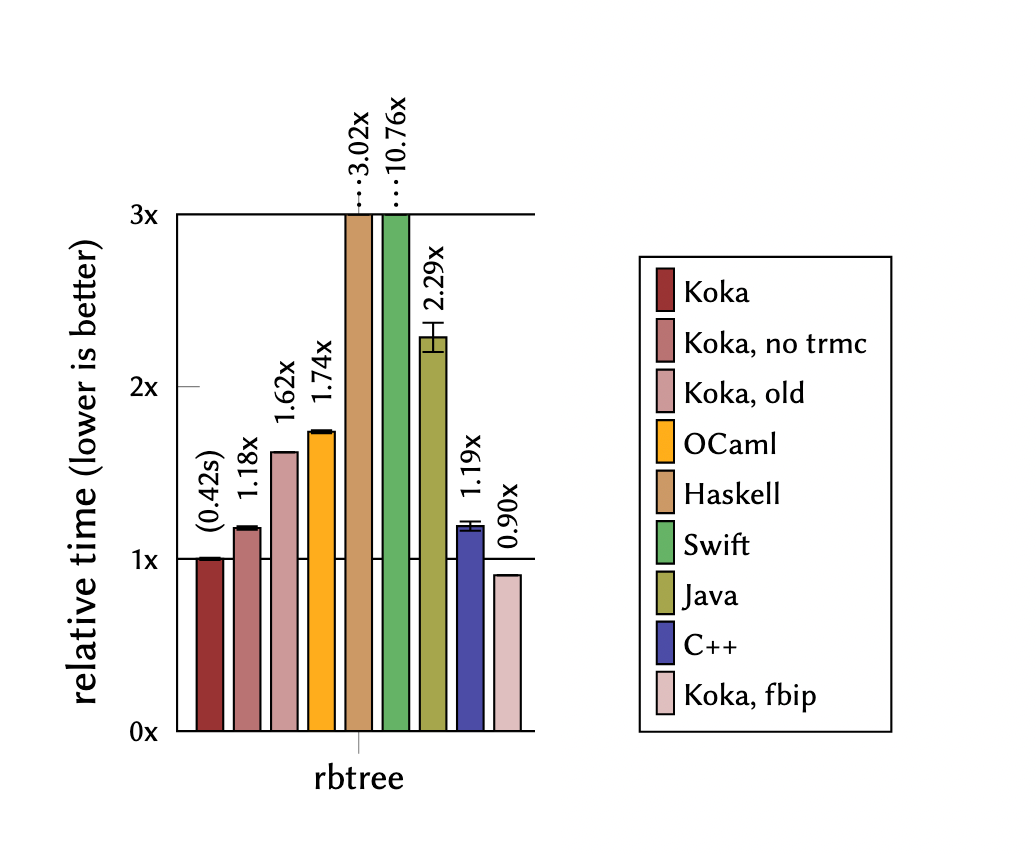
\includegraphics[width=8cm]{rbtree.png}
% % % \end{center}
% % % \end{frame}

% % \begin{frame}[fragile]{Link-inverted tree traversal}
% % \begin{code}
% % fun map(t : tree<a>, f : a -> b) : tree<b>
  % % down(t, f, Top)

% % fun down(t, f, z)
  % % match(t)
    % % Bin(l, x, r) -> down(l, f, BinL(z, x, r))
    % % Tip -> up(Tip, f, z)

% % fun up(t, f, z)
  % % match(z)
    % % BinL(z', x, r)
      % % -> down(r, f, BinR(t, f(x), z'))
    % % BinR(l, x, z') -> up(Bin(l, x, t), f, z')
    % % Top -> t
% % \end{code}
% % \end{frame}

% % \begin{frame}{Conclusion}
    % % Stackless algorithms can be {\raise.17ex\hbox{$\scriptstyle\sim$}}10\% faster\\

    % % They can often be derived by the CPS transform\\

    % % With reuse analysis they are easy to implement\\
% % \end{frame}

\end{document}